\doublespacing
\chapter{Supplementary Information for Chapter~\ref{ch:CoBS}}
\label{appendix: CoBS}
\acresetall


\section{Coupled-Wave Equations}
\label{Appendix:Coupled-Wave Equations}

Here we derive the coupled wave equations that describe Coherently stimulated Brillouin Scattering (\acs{CoBS}) involving a pump, Stokes, probe, and backscattered optical field given respectively by
\\
\begin{equation}
    \tilde{E}_{P}(z,t) = A_{P}e^{i(k_{P}z - \omega_{P}t)} + c.c.,
    \label{eq:Pump optical field}
\end{equation}
\\
\begin{equation}
    \tilde{E}_{S}(z,t) = A_{S}e^{i(-k_{S}z - \omega_{S}t)} + c.c.,
    \label{eq:Stokes optical field}
\end{equation}
\\
\begin{equation}
    \tilde{E}_{Pr}(z,t) = A_{Pr}e^{i(k_{Pr}z - \omega_{Pr}t)} + c.c.,
    \label{eq:Probe optical field}
\end{equation}
\\
\begin{equation}
    \tilde{E}_{Sig}(z,t) = A_{Sig}e^{i(-k_{Sig}z - \omega_{Sig}t)} + c.c.,
    \label{eq:Signal optical field}
\end{equation}
\\
\noindent and a common acoustic field given by
\\
\begin{equation}
    \tilde{\rho}(z,t) = \rho_{0} + \rho(z,t)e^{i(qz - \Omega t)} + c.c.,
    \label{eq:acoustic field}
\end{equation}
\\
\noindent where \(\Omega = \omega_{P} - \omega_{S}\) and \(q = k_{P} - k_{S} \approx 2k_{P}\).


\subsection{Acoustic Field}
\label{Coupled-Wave Equations:Acoustic Field}

As in the case of SBS\cite{boyd2020nonlinear}, we start by assuming that the material obeys the acoustic wave equation,
\\
\begin{equation}
    \frac{\partial^{2}\tilde{\rho}}{\partial t^{2}} - \Gamma^{\prime}\nabla^{2}\frac{\partial\tilde{\rho}}{\partial t} - v_{s}^{2}\nabla^{2}\tilde{\rho} = \nabla\cdot\vec{f},
    \label{eq:acoustic wave equation}
\end{equation}
\\
\noindent where \(v_{s}\) is the sound speed in the material and \(\Gamma^{\prime}\) is a damping parameter given by
\\
\begin{equation}
    \Gamma^{\prime} = \frac{1}{\rho}\left[\frac{4}{3}\eta_{s} + \eta_{b} + \frac{\kappa}{C_{p}}(\gamma - 1)\right],
\end{equation}
\\
\noindent where \(\eta_{s}\) and \(\eta_{b}\) are the shear and bulk viscosity coefficients of the material, respectively. The source term on the right side of Equation~\ref{eq:acoustic wave equation} is the divergence of the electrostrictive force:
\\
\begin{equation}
    \vec{f} = \nabla p_{st} = \nabla \cdot \Bigg[-\frac{1}{2}\epsilon_{0}\gamma_{e}\Big(\langle\tilde{E}_{P} \cdot \tilde{E}_{S}\rangle + \langle\tilde{E}_{Pr} \cdot \tilde{E}_{Sig}\rangle\Big)\Bigg],
\end{equation}
\\
which yields, assuming the acoustic wave varies slowly in time,
\\
\begin{equation}
    \nabla\cdot\vec{f} = \epsilon_{0}\gamma_{e}q^{2}(A_{P}A_{S}^{*} + A_{Pr}A_{Sig}^{*})e^{i\Delta kz},
    \label{eq:electrostrictive force term}
\end{equation}
\\
where \(\Delta k = (k_{Pr} - k_{Sig}) - (k_{P} - k_{S})\) is the phase mismatch between the four optical fields. Only two electrostrictive terms survive after accounting for the orthogonal polarization of the pump and Stokes fields with respect to that of the probe and backscattered signal. Inserting this electrostrictive force term (Equation~\ref{eq:electrostrictive force term}) and the acoustic field (Equation~\ref{eq:acoustic field}) into the acoustic wave equation (Equation~\ref{eq:acoustic wave equation}), we find
\\
\begin{equation}
    -2i\Omega\frac{\partial\rho}{\partial t} - \Gamma^{\prime}2iq^{2}\Omega\rho - 2iqv_{s}^{2}\frac{\partial\rho}{\partial z} = \epsilon_{0}\gamma_{e}q^{2}(A_{P}A_{S}^{*} + A_{Pr}A_{Sig}^{*})e^{i\Delta kz},
\end{equation}
\\
which can be restated in terms of the Brillouin linewidth, \(\Gamma_{B} = q^{2}\Gamma^{\prime}\), as
\\
\begin{equation}
    -2i\Omega\frac{\partial\rho}{\partial t} - 2i\Omega\Gamma_{B}\rho - 2iqv_{s}^{2}\frac{\partial\rho}{\partial z} = \epsilon_{0}\gamma_{e}q^{2}(A_{P}A_{S}^{*} + A_{Pr}A_{Sig}^{*})e^{i\Delta kz}.
    \label{eq:in terms of Brillouin linewidth}
\end{equation}
\\
Given the phonon dispersion relations \(\Omega_{B} = |q_{B}|v_{s}\) and \(\Omega^{2} = q^{2}\left(v_{s}^{2} - i\Omega\Gamma^{\prime}\right)\), Equation~\ref{eq:in terms of Brillouin linewidth} can be rewritten as
\\
\begin{equation}
    -2i\Omega\frac{\partial\rho}{\partial t} + \left(\Omega_{B}^{2} - \Omega^{2} - i\Omega\Gamma_{B}\right)\rho - 2iqv_{s}^{2}\frac{\partial\rho}{\partial z} = \epsilon_{0}\gamma_{e}q^{2}(A_{P}A_{S}^{*} + A_{Pr}A_{Sig}^{*})e^{i\Delta kz}.
    \label{eq:in terms of Omega_B}
\end{equation}
\\
We take the common assumption that the phonon propagation distance is small compared to the distance over which the source term varies significantly, which allows the spatial derivative term in Equation~\ref{eq:in terms of Omega_B} to be dropped. We further assume steady-state conditions such that the time derivative term also vanishes, leaving
\\
\begin{equation}
    (\Omega^{2}_{B} - \Omega^{2} - i\Omega\Gamma_{B})\rho = \epsilon_{0}\gamma_{e}q^{2}(A_{P}A_{S}^{*} + A_{Pr}A_{Sig}^{*})e^{i\Delta kz}.
\end{equation}
\\
We thus find the acoustic field amplitude to be
\\
\begin{equation}
    \rho(z,t) = \epsilon_{0}\gamma_{e}q^{2}\frac{(A_{P}A_{S}^{*} + A_{Pr}A_{Sig}^{*})e^{i\Delta kz}}{\Omega_{B}^{2} - \Omega^{2} - i\Omega\Gamma_{B}}.
    \label{eq:Acoustic field amplitude}
\end{equation}


\subsection{Optical Fields}
\label{Coupled-Wave Equations:Optical Fields}

We now turn to the spatial evolution of the optical fields, described by the wave equation,
\\
\begin{equation}
    \frac{\partial^{2}\tilde{E}_{i}}{\partial z^{2}} - \frac{n^{2}}{c^{2}}\frac{\partial^{2}\tilde{E}_{i}}{\partial t^{2}} = \frac{1}{\epsilon_{0}c^{2}}\frac{\partial^{2}\tilde{P}_{i}}{\partial t^{2}},
    \label{eq:Wave equation}
\end{equation}
\\
where \(i\) denotes the four optical fields, namely: pump, Stokes, probe, and the backscattered signal. The total nonlinear polarization that gives rise to the source term in the wave Equation~is given by
\\
\begin{equation}
    \tilde{P} = \epsilon_{0}\Delta\chi\tilde{E} = \epsilon_{0}\Delta\epsilon\tilde{E} = \epsilon_{0}\rho^{-1}\gamma_{e}\tilde{\rho}\tilde{E}.
\end{equation}
\\
The parts of \(\tilde{P}\) that can act as phase-matched source terms for the optical fields are
\\
\begin{equation}
    \tilde{P}_{P} = p_{P}e^{i(k_{P}z - \omega_{P} t)} + c.c. = \frac{1}{2}\epsilon_{0}\rho_{0}^{-1}\gamma_{e}\rho A_{S}e^{i(k_{P}z - \omega_{P} t)},
    \label{eq:Pump phase-matched source term}
\end{equation}
\\
\begin{equation}
    \tilde{P}_{S} = p_{S}e^{i(-k_{S}z - \omega_{S} t)} + c.c. = \frac{1}{2}\epsilon_{0}\rho_{0}^{-1}\gamma_{e}\rho^{*} A_{P}e^{i(-k_{S}z - \omega_{S} t)},
    \label{eq:Stokes phase-matched source term}
\end{equation}
\\
\begin{equation}
    \tilde{P}_{Pr} = p_{Pr}e^{i(k_{Pr}z - \omega_{Pr} t)} + c.c. = \frac{1}{2}\epsilon_{0}\rho_{0}^{-1}\gamma_{e}\rho A_{Sig}e^{i(k_{Pr}z - \omega_{Pr} t)}e^{i\Delta kz},
    \label{eq:Probe phase-matched source term}
\end{equation}
\\
\begin{equation}
    \tilde{P}_{Sig} = p_{Sig}e^{i(-k_{Sig}z - \omega_{Sig} t)} + c.c. = \frac{1}{2}\epsilon_{0}\rho_{0}^{-1}\gamma_{e}\rho^{*} A_{Pr}e^{i(-k_{Sig}z - \omega_{Sig} t)}e^{-i\Delta kz}.
    \label{eq:Signal phase-matched source term}
\end{equation}
\\
Inserting the optical fields (Equations~\ref{eq:Pump optical field}-\ref{eq:Signal optical field}) and phase-matched source terms (Equations~\ref{eq:Pump phase-matched source term}-\ref{eq:Signal phase-matched source term}) into Equation~\ref{eq:Wave equation}, we obtain
\\
\begin{equation}
    \frac{\partial A_{P}}{\partial z} + \frac{n}{c}\frac{\partial A_{P}}{\partial t} = \frac{i\omega_{P}\gamma_{e}}{2nc\rho_{0}}\rho A_{2},
\end{equation}
\\
\begin{equation}
    -\frac{\partial A_{S}}{\partial z} + \frac{n}{c}\frac{\partial A_{S}}{\partial t} = \frac{i\omega_{S}\gamma_{e}}{2nc\rho_{0}}\rho^{*}A_{P},
\end{equation}
\\
\begin{equation}
    \frac{\partial A_{Pr}}{\partial z} + \frac{n}{c}\frac{\partial A_{Pr}}{\partial t} = \frac{i\omega_{Pr}\gamma_{e}}{2nc\rho_{0}}\rho A_{Sig},
\end{equation}
\\
\begin{equation}
    -\frac{\partial A_{Sig}}{\partial z} + \frac{n}{c}\frac{\partial A_{Sig}}{\partial t} = \frac{i\omega_{Sig}\gamma_{e}}{2nc\rho_{0}}\rho^{*}A_{Pr},
\end{equation}
\\
We again assume steady-state conditions, allowing the time derivative term to be dropped. Plugging in the acoustic field amplitude (Equation~\ref{eq:Acoustic field amplitude}), we arrive at the coupled-amplitude wave equations for the optical fields,
\\
\begin{equation}
    \frac{\partial A_{P}}{\partial z} = \frac{i\epsilon_{0}\omega_{P} q^{2}\gamma_{e}^{2}}{2nc\rho_{0}}\frac{(A_{P}|A_{S}|^{2} + A_{Pr}A_{Sig}^{*}A_{S})e^{i\Delta kz}}{\Omega_{B}^{2} - \Omega^{2} - i\Omega\Gamma_{B}},
    \label{eq:Pump coupled-amplitude wave equation}
\end{equation}
\\
\begin{equation}
    \frac{\partial A_{S}}{\partial z} = -\frac{i\epsilon_{0}\omega_{S} q^{2}\gamma_{e}^{2}}{2nc\rho_{0}}\frac{(|A_{P}|^{2}A_{S}^{*} + A_{Pr}A_{Sig}^{*}A_{P})e^{-i\Delta kz}}{\Omega_{B}^{2} - \Omega^{2} + i\Omega\Gamma_{B}},
\end{equation}
\\
\begin{equation}
    \frac{\partial A_{Pr}}{\partial z} = \frac{i\epsilon_{0}\omega_{Pr} q^{2}\gamma_{e}^{2}}{2nc\rho_{0}}\frac{(A_{P}A_{S}^{*}A_{Sig} + A_{Pr}|A_{Sig}|^{2})e^{i\Delta kz}}{\Omega_{B}^{2} - \Omega^{2} - i\Omega\Gamma_{B}},
\end{equation}
\\
\begin{equation}
    \frac{\partial A_{Sig}}{\partial z} = -\frac{i\epsilon_{0}\omega_{Sig} q^{2}\gamma_{e}^{2}}{2nc\rho_{0}}\frac{(A_{P}A_{S}^{*}A_{Pr} + |A_{Pr}|^{2}A_{Sig}^{*})e^{-i\Delta kz}}{\Omega_{B}^{2} - \Omega^{2} + i\Omega\Gamma_{B}}.
    \label{eq:Signal coupled-amplitude wave equation}
\end{equation}
\\
We drop the very small signal amplitude terms on the right side of Equations~\ref{eq:Pump coupled-amplitude wave equation}-\ref{eq:Signal coupled-amplitude wave equation} and integrate each along the effective length to get the amplitudes,
\\
\begin{equation}
  A_{P} = \frac{i\epsilon_{0}\omega_{P}q^{2}\gamma_{e}^{2}}{2nc\rho_{0}}\frac{A_{P}|A_{S}|^{2}}{\Omega_{B}^{2} - \Omega^{2} - i\Omega\Gamma_{B}} \frac{e^{i\Delta kL} - 1}{i\Delta k},
\end{equation}
\\
\begin{equation}
  A_{S} = -\frac{i\epsilon_{0}\omega_{S}q^{2}\gamma_{e}^{2}}{2nc\rho_{0}}\frac{|A_{P}|^{2}A_{S}^{*}}{\Omega_{B}^{2} - \Omega^{2} + i\Omega\Gamma_{B}} \frac{e^{-i\Delta kL} - 1}{-i\Delta k},
\end{equation}
\\
\begin{equation}
  A_{Pr} = \frac{i\epsilon_{0}\omega_{Pr}q^{2}\gamma_{e}^{2}}{2nc\rho_{0}}\frac{A_{P}A_{S}^{*}A_{Sig}}{\Omega_{B}^{2} - \Omega^{2} - i\Omega\Gamma_{B}} \frac{e^{i\Delta kL} - 1}{i\Delta k},
\end{equation}
\\
\begin{equation}
  A_{Sig} = -\frac{i\epsilon_{0}\omega_{Sig}q^{2}\gamma_{e}^{2}}{2nc\rho_{0}}\frac{A_{P}A_{S}^{*}A_{Pr}}{\Omega_{B}^{2} - \Omega^{2} + i\Omega\Gamma_{B}} \frac{e^{-i\Delta kL} - 1}{-i\Delta k}.
  \label{eq:Signal amplitude}
\end{equation}
\\
We focus on the signal amplitude given by Equation~\ref{eq:Signal amplitude}, noting that close to resonance, the denomenator of the middle term containing \(\Omega\) can be approximated as,
\\
\begin{equation}
\Omega_{B}^{2} - \Omega^{2} + i\Omega\Gamma_{B} \approx \Omega_{B}(\Omega - \Omega_{B} + i\Gamma_{B}),
\end{equation}
\\
giving
\\
\begin{equation}
  A_{Sig} = -\frac{i\epsilon_{0}\omega_{Sig}q^{2}\gamma_{e}^{2}}{2nc\rho_{0}}\frac{A_{P}A_{S}^{*}A_{Pr}}{\Omega_{B}(\Omega - \Omega_{B} + i\Gamma_{B})} \frac{e^{-i\Delta kL} - 1}{-i\Delta k},
  \label{eq:resonance}
\end{equation}
\\
and in fact on resonance the expression reduces to
\\
\begin{equation}
  A_{Sig} = -\frac{i\epsilon_{0}\omega_{Sig}q^{2}\gamma_{e}^{2}}{2nc\rho_{0}}\frac{A_{P}A_{S}^{*}A_{Pr}}{\Omega_{B}i\Gamma_{B}} \frac{e^{-i\Delta kL} - 1}{-i\Delta k}.
\end{equation}
\\
Using \(q = 2k_{P} = 2\omega n/c\) and \(q = \Omega_{B}/v_{s}\), we can express the leading terms as
\\
\begin{equation}
  A_{Sig} = -\frac{\epsilon_{0}\omega^{2}\gamma_{e}^{2}}{c^{2}v_{s}\rho_{0}\Gamma_{B}}A_{P}A_{S}^{*}A_{Pr} \frac{e^{-i\Delta kL} - 1}{-i\Delta k},
\end{equation}
\\
where we have dropped the signal designator on \(\omega\). Defining the Brillouin gain factor, \(g_{0}\), as Boyd does,
\\
\begin{equation}
  g_{0} = \frac{\gamma_{e}^{2}\omega^{2}}{nv_{s}c^{3}\rho_{0}\Gamma_{B}},
\end{equation}
reduces this expression to
\\
\begin{equation}
  A_{Sig} = -\epsilon_{0}ncg_{0}A_{P}A_{S}^{*}A_{Pr} \frac{e^{-i\Delta kL} - 1}{-i\Delta k}.
\end{equation}
\\
The intensity of the backscattered signal is given by the magnitude of the time-averaged Poynting vector, given by
\\
\begin{equation}
  I_{i} = 2n\epsilon_{0}c|A_{i}|^{2}, \qquad i = 1,2,3,...
\end{equation}
\\
which produces for the signal intensity
\\
\begin{equation}
  I_{Sig} = 2\epsilon_{0}nc(\epsilon_{0}ncg_{0})^{2}|A_{P}|^{2}|A_{S}^{*}|^{2}|A_{Pr}|^{2}\left|\frac{e^{-e\Delta kL} - 1}{-i\Delta k}\right|^{2}
  = 2\epsilon_{0}^{3}\epsilon_{0}n^{3}c^{3}g_{0}^{2}\frac{I_{P}}{2\epsilon_{0}nc}\frac{I_{S}}{2\epsilon_{0}nc}\frac{I_{Pr}}{2\epsilon_{0}nc}\left|\frac{e^{-e\Delta kL} - 1}{-i\Delta k}\right|^{2}.
\end{equation}
\\
The squared modulus term containing \(\Delta k\) can be reduced as
\\
\begin{gather}
  \bigg|\frac{e^{-i\Delta kL} - 1}{-i\Delta k}\bigg|^{2} = \frac{(e^{-i\Delta kL} - 1)(e^{i\Delta kL} - 1)}{(\Delta k)^{2}} = \frac{L^{2}}{(\Delta kL)^{2}}\Bigg[ 2 - 2\Bigg(\frac{e^{i\Delta kL} + e^{-1\Delta kL}}{2}\Bigg)\Bigg] \notag \\ \notag \\
  = \frac{2L^{2}(1 - cos\Delta kL)}{(\Delta kL)^{2}} = \frac{4L^{2}sin^{2}\big(\frac{\Delta kL}{2}\big)}{\big(\Delta kL\big)^{2}} = \frac{L^{2}sin^{2}\big(\frac{\Delta kL}{2}\big)}{\big(\frac{\Delta kL}{2}\big)^{2}} = L^{2}sinc^{2}\bigg(\frac{\Delta kL}{2}\bigg),
\end{gather}
\\
giving as a final expression for backscattered signal intensity,
\\
\begin{equation}
I_{Sig} = \frac{1}{4}(g_{0}L)^{2}I_{P}I_{S}I_{Pr}sinc^{2}\left(\frac{\Delta kL}{2}\right).
\end{equation}
\\

To find the power of the backscattered signal, we would integrate this intensity over the effective area. For a uniform area \(A_{eff}\), this gives
\\
\begin{equation}
  P_{Sig} = I_{Sig}A_{eff} = \frac{1}{4}(g_{0}L)^{2}\frac{A_{eff}}{A_{eff}}I_{P}\frac{A_{eff}}{A_{eff}}I_{S}\frac{A_{eff}}{A_{eff}}I_{Pr}sinc^{2}\left(\frac{\Delta kL}{2}\right)A_{eff},
\end{equation}
\\
or,
\\
\begin{equation}
  P_{Sig} = \frac{1}{4}(G_{B}L)^{2}P_{P}P_{S}P_{Pr}sinc^{2}\left(\frac{\Delta kL}{2}\right),
\end{equation}
\\
where,
\\
\begin{equation}
  G_{B} = \frac{g_{0}}{A_{eff}}.
\end{equation}
\\
It can be seen that off resonance, the \(\Omega\) term from Equation~\ref{eq:resonance} goes to a lorentzian form after taking the squared modulus for intensity.

\newpage

%------------------------------------------------------------------------------%

\section{Scattered Power Comparison to Traditional Brillouin Scattering Processes}
\label{appendix:comparison}

This appendix provides a comparative analysis of the scattered power produced by our instrument to that of standard Brillouin scattering processes-that is, spontaneous and stimulated Brillouin scattering. The difference in behavior of our instrumdent from the traditional techniques arises due to the coherent stimulation of the acoustic mode by the pump and Stokes fields, producing a 4-wave-coupled-amplitude interaction that yields much higher scattered powers in smaller lengths. While our instrument is particularly well suited to small interaction lengths due to enhanced phase-matching relaxation, it maintains production of a significant amount of scatterd power at greater lengths as well (greater than \SI{1}{\meter}). This is because the reduction in scattered power from the breakdown of phase-matching relaxation at greater lengths is perfectly counter-balanced by the quadradic dependence on length in the overall scatterd power, as seen in Equation~\ref{Eq:Theoretical Framework:Scattered Power}. At very large lengths (greater than \SI{1}{\kilo\meter}), the instrument is ultimately limited by the coherence length of the lasers employed, as the process relies on the coherent stimulation of the phonon mode and thus the mutual coherence of the pump and Stokes fields over the interaction length. Here we offer an exploration into the respective performance of each technique across the entire meaningful length scale, from nanometers to kilometers.

Despite shared dependence on basic Brillouin scattering principles, the three techniques compared here (spontaneous-, stimulated-, and coherently stimulated Brillouin scattering) yield significantly different scattered power for identical experimental paramters. At small lengths, the high-gain threshold for optical stimulation of the material fluctuations is often not achievable without the use of extremely large optical powers. This prevents the system from entering a process of exponential growth of the scattered Stokes light indicative of stimulated Brillouin scattering.\cite{boyd2020nonlinear} In this low-gain regime, any scattered Stokes light is spontanously scattered from thermal fluctuations of the material, or from quantum-mechanical fluctuations of materials at the ground state. The low-gain regime is defined by an overall process gain factor, denoted by \(G = G_{\mathrm{P}}P_{\mathrm{P}}L\), which is much less than unity (\(G \ll 1\)). Here, \(G_{\mathrm{B}}\) is the effective Brillouin gain in \si{\per\watt\per\meter} (\(G_{\mathrm{B}} = \frac{g}{A_{\mathrm{eff}}}\)), \(P_{\mathrm{P}}\) is the pump power, and \(L\) is the effective length. This spontaneous scattering process follows a linear growth trend described by Boyd et al in 1990 \cite{boyd1990noise} as

\begin{equation}
  R = \frac{\langle|E_{\mathrm{S}}|^{2}\rangle}{\langle|E_{\mathrm{P}}|^{2}\rangle} = (\bar{n} + 1)g\hbar\omega_{\mathrm{S}}\Gamma_{\mathrm{B}}\frac{L}{4A_{\mathrm{eff}}},
\end{equation}

where R is the reflectivity, or the ratio of scattered Stokes intensity to incident pump intensity, and \(\bar{n} = (e^{\frac{\hbar\Omega_{\mathrm{B}}}{k_{\mathrm{B}}T}} - 1)^{-1}\) is the mean number of phonons occupying the mode due to thermal fluctuations of the material. Rearranging this Equation and converting to effective Brillouin gain, \(G_{\mathrm{B}}\), and power by applying the effective area, we arrive at the scattered power of the Stokes spontaneous Brillouin scattering process,

\begin{equation}
  P_{\mathrm{S}} = \frac{1}{4}G_{\mathrm{B}}P_{\mathrm{P}}L\hbar\omega_{\mathrm{S}}\Gamma_{\mathrm{B}}(\bar{n} + 1).
  \label{eq:SponBSnbar}
\end{equation}

At room temperature and typical Brillouin frequencies in the GHz range, the quantity \(k_{\mathrm{B}}T \gg \hbar\Omega_{\mathrm{B}}\), allowing

\begin{equation}
e^{\frac{\hbar\Omega_{\mathrm{B}}}{k_{\mathrm{B}}T}} \approx 1 + \frac{\hbar\Omega_{\mathrm{B}}}{k_{\mathrm{B}}T}
\end{equation}

to be a good approximation. We thus find that

\begin{equation}
(\bar{n} + 1) \approx \bar{n} \approx \frac{k_{\mathrm{B}}T}{\hbar\Omega_{\mathrm{B}}}.
\end{equation}

Inserting this reduced quantity into Equation~\ref{eq:SponBSnbar}, we arrive at a convenient expression for the scattered power of the Stokes spontaneous Brillouin scattering process,

\begin{equation}
  P_{S, \,\textit{SponBS}} = \frac{G_{\mathrm{B}}P_{\mathrm{P}}L\omega_{\mathrm{S}}\Gamma_{\mathrm{B}}k_{\mathrm{B}}T}{4\Omega_{\mathrm{B}}}.
  \label{eq:sponBSscatteredPower}
\end{equation}

It may be noted that the derived expression for the low-gain spontaneous regime here matches the form reported by Kharel et al. in 2016 \cite{kharel2016noise} for the complementary forward scattering process. While our backward scattering geometry differs from the forward scattering geometry discussed by Kharel et al., the underlying physics of light coupling to thermally excited acoustic modes is the same..

Next we turn to the high-gain regime leading to a stimulated Brillouin scattering process. This regime is defined by an overall process gain factor, \(G = G_{\mathrm{P}}P_{\mathrm{P}}L\), that is much greater than unity (\(G \gg 1\)). For organic liquids, this crossover threshold from spontaneous to stimulated regimes occurs in the range of \(20 < G < 25\), \cite{boyd1990noise} whereas for typical lengths of single mode fiber it can be lower \cite{ippen1972stimulated} owing to the small effective area compared to longer effective lengths of fiber typically used.

The reflectivity of a stimulated Brillouin scattering process in the high-gain regime is given by \cite{boyd1990noise}

\begin{equation}
  R = \frac{\langle|E_{\mathrm{S}}|^{2}\rangle}{\langle|E_{\mathrm{P}}|^{2}\rangle} = \frac{Y}{\sqrt{\pi}}\frac{e^{G}}{G^{\frac{3}{2}}},
\end{equation}

where \(Y\) is the reflectivity of the low-gain (spontaneous) regime given above and \(G\) is the overall process gain factor, \(G = G_{\mathrm{P}}P_{\mathrm{P}}L\). Again, converting to the effective Brillouin gain, \(G_{\mathrm{B}}\), and power by applying the effective area, we solve for the scattered power of the Stokes field,

\begin{equation}
  P_{\mathrm{S,\,StimBS}} = \frac{G_{\mathrm{B}}P_{\mathrm{P}}L\omega_{\mathrm{S}}\Gamma_{\mathrm{B}}k_{\mathrm{B}}T}{4\sqrt{\pi}\Omega_{\mathrm{B}}}\frac{e^{G}}{G^{\frac{3}{2}}}
  \label{eq:StimBSUndepletedPump}
\end{equation}

This expression captures the exponential growth in scattered power as any parameter within the overall process gain factor, \(G = G_{\mathrm{B}}P_{\mathrm{P}}L\), increases. However, this exponential growth can only continue while the pump is not significantly undepleted. Once the scattered power described by Equation~\ref{eq:StimBSUndepletedPump} grows to a significant fraction of the driving pump power, the exponential increase in scattered Stokes power asymptotically approaches the pump power. For very large \(G\), virtually all of the pump energy is converted to scattered Stokes energy in a complete transfer process.\cite{boyd2020nonlinear} To account for pump depletion, we numerically solve the transendental Equation~derived in Boyd's Nonlinear Optics which describes the effects of pump depletion, given here in terms of power as

\begin{equation}
  P_{\mathrm{S}}(L) = \frac{P_{\mathrm{S}}(0)x(1 - x)}{e^{G_{\mathrm{B}}P_{\mathrm{P}}(0)L(1 - x)} - x},
\end{equation}

where \(x = P_{\mathrm{S}}(0)/P_{\mathrm{P}}(0)\), or the ratio of the unknown Stokes power at the end of its journey through the medium (\(z=0\)) to the known pump power at the beginning (also \(z=0\)). This solution for \(x\), specific to system parameters such as length, offers via its definition the solution to the unknown power of the scattered Stokes light at the end of its traversal through the effective length, given as

\begin{equation}
  P_{\mathrm{S}}(0) = xP_{\mathrm{P}}(0).
\end{equation}

The solution to this numeric approach to scattered power in the high-gain (stimulated) Brillouin scattering regime with pump depletion effects at large \(G\) is plotted for varying effective lengths in Figure~\ref{fig:SponBSvsStimBSvsCoBS}, along with the analytical solutions derived previously for the low-gain (spontaneous) regime and our coherently stimulated Brillouin spectrometer (\acs{CoBS}) given by Equation~\ref{Eq:Theoretical Framework:Scattered Power}. System parameters used to generate the plot for each of the three processes are provided in Tables \ref{tab:CoBS Parameters} and \ref{tab:SBS Parameters}. Wherever possible, the parameters shared by all three Brillouin scattering processes were kept consistent, while quantities unique to each process were assigned their respective values.

\begin{table}[ht]
  \centering
  \caption[Parameters relevant to the \acs{CoBS} process for the example \ac{UHNA3} fiber.]{Parameters relevant to the \acs{CoBS} process for the example \ac{UHNA3} fiber. \(G_{\mathrm{B}}\) is the effective Brillouin gain, \(P_{\mathrm{P}}\) is the pump power, \(P_{\mathrm{S}}\) is the Stokes power, \(P_{\mathrm{Pr}}\) is the probe power, and \(\Delta\lambda\) is the wavelength detuning of the probe from the pump.}
  \textbf{Coherently Stimulated Brillouin Scattering Process Model System Parameters}
  \renewcommand{\arraystretch}{1.2}
  \begin{tabular}{c c c c c}
    \toprule
    \multicolumn{1}{c}{\(\mathbf{G_{\mathrm{\textbf{B}}}}\)} &
    \multicolumn{1}{c}{\(\mathbf{P_{\mathrm{\textbf{P}}}}\)} &
    \multicolumn{1}{c}{\(\mathbf{P_{\mathrm{\textbf{S}}}}\)} &
    \multicolumn{1}{c}{\(\mathbf{P_{\mathrm{\textbf{Pr}}}}\)} &
    \multicolumn{1}{c}{\(\mathbf{\Delta\lambda}\)} \\
    \multicolumn{1}{c}{(\si{\per\watt\per\meter})} &
    \multicolumn{1}{c}{(\si{\watt})} &
    \multicolumn{1}{c}{(\si{\watt})} &
    \multicolumn{1}{c}{(\si{\watt})} &
    \multicolumn{1}{c}{(\si{\pico\meter})} \\

    \midrule
    \num{0.6} & \num{1} & \num{1} & \num{1} & \num{20} \\
    \bottomrule
  \end{tabular}
  \label{tab:CoBS Parameters}
\end{table}

\begin{table}[ht]
  \centering
  \caption[Parameters relevant to the spontaneous and/or stimulated backward Brillouin scattering processes for the example \ac{UHNA3} fiber.]{Parameters relevant to the spontaneous and/or stimulated backward Brillouin scattering processes for the example \ac{UHNA3} fiber. \(G_{\mathrm{B}}\) is the Brillouin gain coefficient, \(P_{\mathrm{P}}\) is the pump power, \(\omega\) is the optical angular frequency, \(\Gamma_{\mathrm{B}}\) is the acoustic damping rate, \(k_{\mathrm{B}}\) is Boltzmann's constant, \(T\) is the temperature, and \(\Omega_{\mathrm{B}}\) is the acoustic angular frequency.}
  \textbf{Spontaneous and Stimulated Scattering Process Model System Parameters}
  \renewcommand{\arraystretch}{1.2}
  \begin{tabular}{c c c c c c c c c}
    \toprule
    \multicolumn{1}{c}{\(\mathbf{G_{\mathrm{\textbf{B}}}}\)} &
    \multicolumn{1}{c}{\(\mathbf{P_{\mathrm{\textbf{P}}}}\)} &
    \multicolumn{1}{c}{\(\mathbf{P_{\mathrm{\textbf{S,seed}}}}\)} &
    \multicolumn{1}{c}{\(\mathbf{n}\)} &
    \multicolumn{1}{c}{\(\mathbf{\lambda_{\mathrm{\textbf{P}}}}\)} &
    \multicolumn{1}{c}{\(\mathbf{\Gamma_{\mathrm{\textbf{B}}}}\)} &
    \multicolumn{1}{c}{\(\mathbf{k_{\mathrm{\textbf{B}}}}\)} &
    \multicolumn{1}{c}{\(\mathbf{T}\)} &
    \multicolumn{1}{c}{\(\mathbf{\Omega_{\mathrm{\textbf{B}}}}\)} \\
    \multicolumn{1}{c}{(\si{\per\watt\per\meter})} &
    \multicolumn{1}{c}{(\si{\watt})} &
    \multicolumn{1}{c}{(\si{\pico\watt})} &
    \multicolumn{1}{c}{} &
    \multicolumn{1}{c}{(\si{\nano\meter})} &
    \multicolumn{1}{c}{(\si{\mega\hertz})} &
    \multicolumn{1}{c}{(\si{\joule\per\kelvin})} &
    \multicolumn{1}{c}{(\si{\kelvin})} &
    \multicolumn{1}{c}{(\si{\giga\hertz})} \\

    \midrule
    \num{0.6} & \num{1} & \num{1} & \num{1.48} & \num{1549} & \(2\pi \cdot 80\) & \num{1.38e-23} & \num{295} & \(2\pi \cdot 9.18\) \\
    \bottomrule
  \end{tabular}
  \label{tab:SBS Parameters}
\end{table}

At lengths beyond a centimeter, the phase-matching relaxation of the \acs{CoBS} process begins to break down, and the specific choice in pump and probe detuning becomes critical. This corresponds to a narrowing of the \(\mathrm{sinc}^{2}\) function given in Equation~\ref{Eq:Phi}. The scattered power beyond this length rises and falls according to the oscillations of the \(\mathrm{sinc}^{2}\) function far from the origin. As length increases continuously beyond \SI{1}{\meter}, the scattered power oscillates with increasing frequency and ceases to offer practical significance. To better visualize the scattered power offered by the instrument in this region, we have computed the envelope of scattered power. In a laboratory setting, the appropriate pump and probe detuning would be selected for the specific sample length being measured such that the scattered power function lies on a local peak of the \(\mathrm{sinc}^{2}\) function.

\begin{figure}[ht]
\centering
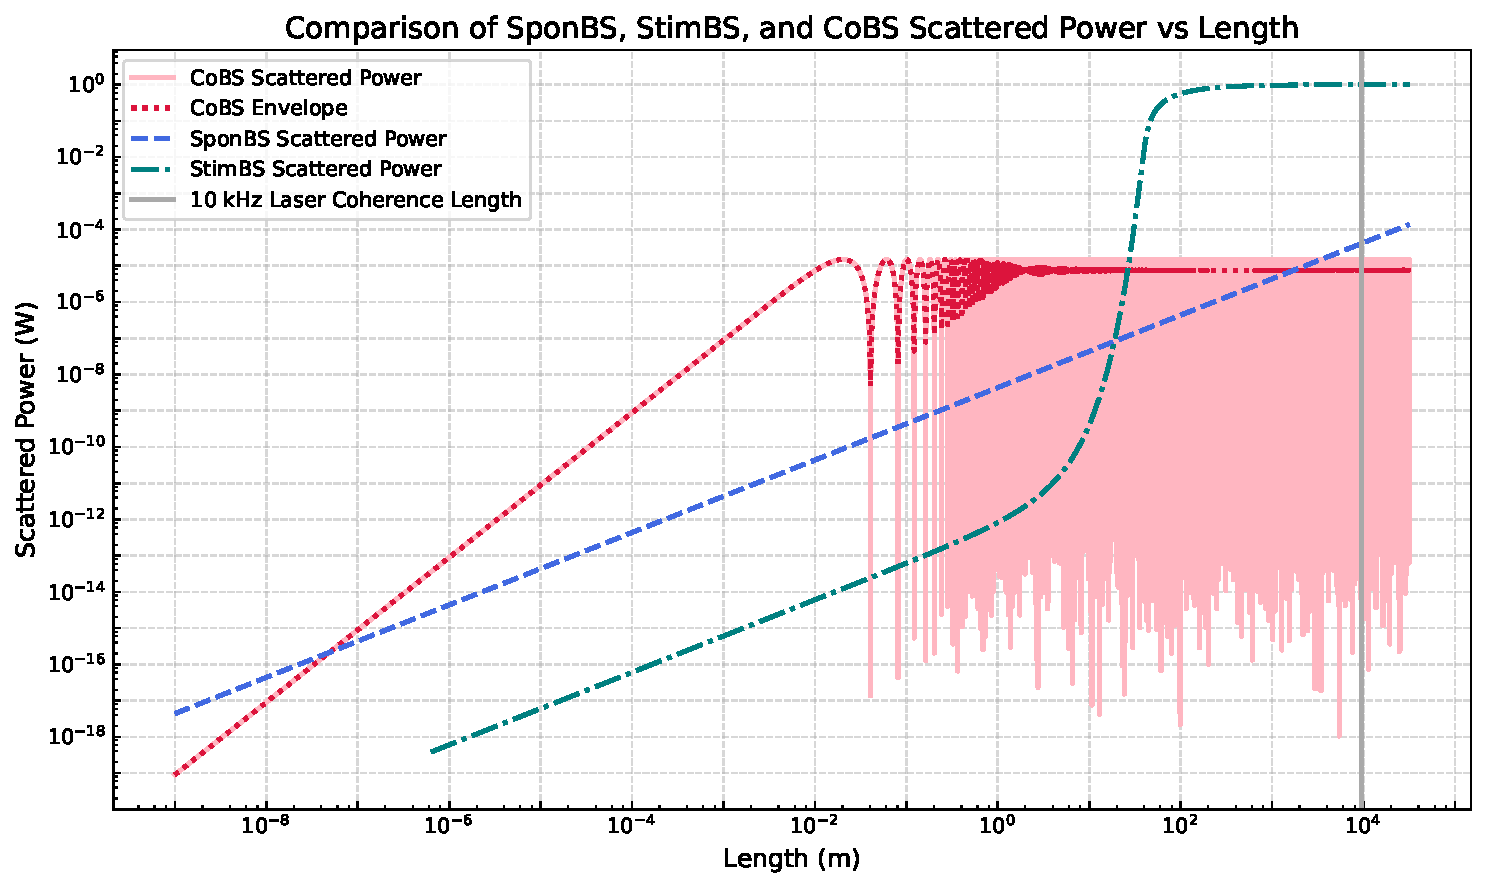
\includegraphics[width=\textwidth]{figs/3-CoBS/SponBSvsStimBSvsCoBS.pdf}
\caption{Comparison of scattered power from traditional Brillouin scattering processes and \acs{CoBS}.}
\label{fig:SponBSvsStimBSvsCoBS}
\end{figure}

Figure~\ref{fig:SponBSvsStimBSvsCoBS} shows the advantage that \acs{CoBS} offers compared to the traditional Brillouin processes for the example medium of \ac{UHNA3} fiber. For lengths up to about \SI{50}{\meter} and down to as low as \SI{100}{\nano\meter}, the coherently stimulated process employed by our instrument offers superior scattered power, with the relative advantage peaking for a length just under \SI{1}{\centi\meter}. At this length, the gain factor \(G\) places the traditional process within the low-gain (spontaneous) regime, and thus the scattered power generated is only on the order of 10s of \si{\pico\watt}. In contrast, the scattered power for the same system offered by our instrument is on the order of 10s of \si{\micro\watt}, exceeding that of the spontenous process by a factor of a million. This is, of course, the most ideal case for this system, however it can be seen from Figure~\ref{fig:SponBSvsStimBSvsCoBS} that \acs{CoBS} offers orders of magnitude more scattered power than either traditional process through a wide range of lengths.

\newpage

%--------------------------------------------------------------------%

\section{Observance of Fano-Resonant Asymmetries at Small Signals}
\label{Appendix:Fano}

In \textit{Fano-Resonant Asymmetries at Small Signals} (Section~\ref{Results:Fano-Resonant Asymmetries at Small Signals} in the main text), we discussed how Fano-type interference can distort Brillouin line shapes in situations where the resonant Brillouin amplitude becomes comparable to the background continuum. We focus here on two experiments~(A and B) that reveal these Fano asymmetries especially clearly. Experiment~A is a measurement series using the same \SI{1}{\centi\meter} \ac{UHNA3} fiber referenced in the main discussion, for which the main text showed only the fitted amplitudes (Figure~\ref{fig:Phase-Match}). Here we show the full spectra, illustrating the emergence of asymmetries at lower amplitude conditions. Experiment~B is a distinct measurement involving a short (\(\sim\)\SI{1}{\milli\meter}) bulk liquid sample of carbon disulfide (\ce{CS2}) that we briefly mentioned in Section~\ref{Results:Fano-Resonant Asymmetries at Small Signals} but did not detail. This experiment was performed specifically to further probe the unexpected Fano-like distortions observed in Experiment~A. In each case, we outline the experimental setup, present the spectra, and highlight the appearance of Fano resonances. These observations corroborate the theoretical discussion of Fano line shapes (Section~\ref{Results:Fano-Resonant Asymmetries at Small Signals}) and provide insight into when and why they are most prominent.

\subsection{Fano Experiment~A: Extended \SI{1}{\centi\meter} UHNA3 Fiber Spectra}
\label{Appendix:Fano:Experiment A}

In Section~\ref{Results} of the main text, we introduced a phase-matching experiment on \SI{1}{\centi\meter} of \ac{UHNA3} fiber in which the pump--probe detuning was varied from \SI{5}{\giga\hertz} to \SI{42}{\giga\hertz} in \SI{0.5}{\giga\hertz} increments. There, we reported only the resulting peak amplitudes, showing how they follow a \(\mathrm{sinc^{2}}\) dependence on detuning (Figure~\ref{fig:Phase-Match} in the main text). However, each measurement in that scan also yields a full Brillouin spectrum—75 in total. Here, we present all 75 spectra to illustrate how the line shape transitions from nearly Lorentzian (when the Brillouin peak amplitude greatly exceeds the background continuum) to distinctly Fano-like (when the two amplitudes are comparable). We used the same setup and procedure described in \textit{Phase Matching Characterization} in Section~\ref{Results} of the main text. As the pump-probe detuning increases, the phase-matching term \(\mathrm{sinc^{2}(\Delta kL/2)}\) oscillates through peaks and troughs, causing the Brillouin peak amplitude to rise and fall. When the amplitude is sufficiently large, the Brillouin mode dominates the continuum and the spectrum appears nearly Lorentzian; when it drops to the order of the background amplitude, strong interference skews the line shape into a Fano-like profile.

Figure~\ref{fig:Joy Division UHNA3} highlights the progressive shift from Lorentzian to asymmetric line shapes. Near \SI{5}{\giga\hertz} detuning (top spectra), the resonant amplitude is large relative to the background, giving a classic Lorentzian peak (\(|q| \to \infty\)) at the resonance frequency (\(\sim\)\SI{9.17}{\giga\hertz}). By contrast, at detunings between \(\sim\)15-\SI{20}{\giga\hertz}, where the \(\mathrm{sinc^{2}}\) factor is near a local minimum, the peak amplitude falls to roughly the same level as the continuum, and Fano interference is observed. Interestingly, as the detuning is increased further, and the amplitude rises again on a subsequent “lobe” of the \(\mathrm{sinc^{2}}\) function, the spectra partly recover a Lorentzian shape. This cyclical behavior persists, with each local maximum yielding a near-Lorentzian profile and each local minimum reintroducing a strong Fano distortion. These observations confirm the relationship between Brillouin peak amplitude and continuum interference described in \textit{Fano-Resonant Asymmetries at Small Signals} in Section~\ref{Results}. When the Brillouin amplitude significantly exceeds the background, the discrete phonon resonance dominates, resulting in little or no asymmetry (\(|q| \to \infty\)). Once the two amplitudes become comparable, Fano interference skews the line shape, shifting the apparent peak frequency slightly and altering the slope on either side of the resonance. Analyzing selected spectra with both Lorentzian and Fano fits indicates that ignoring these distortions can lead to up to a 5–10\% misestimation of peak amplitude in the “trough” (low-amplitude) sets. This underscores the importance of employing a Fano model in small-signal measurements where the Brillouin peak may not tower over the background. A comparative analysis of a Lorentzian vs. Fano fit function applied to highly assymetric spectra is explored in the following section, for data gathered from Experiment~B.

\begin{figure}[ht]
\centering
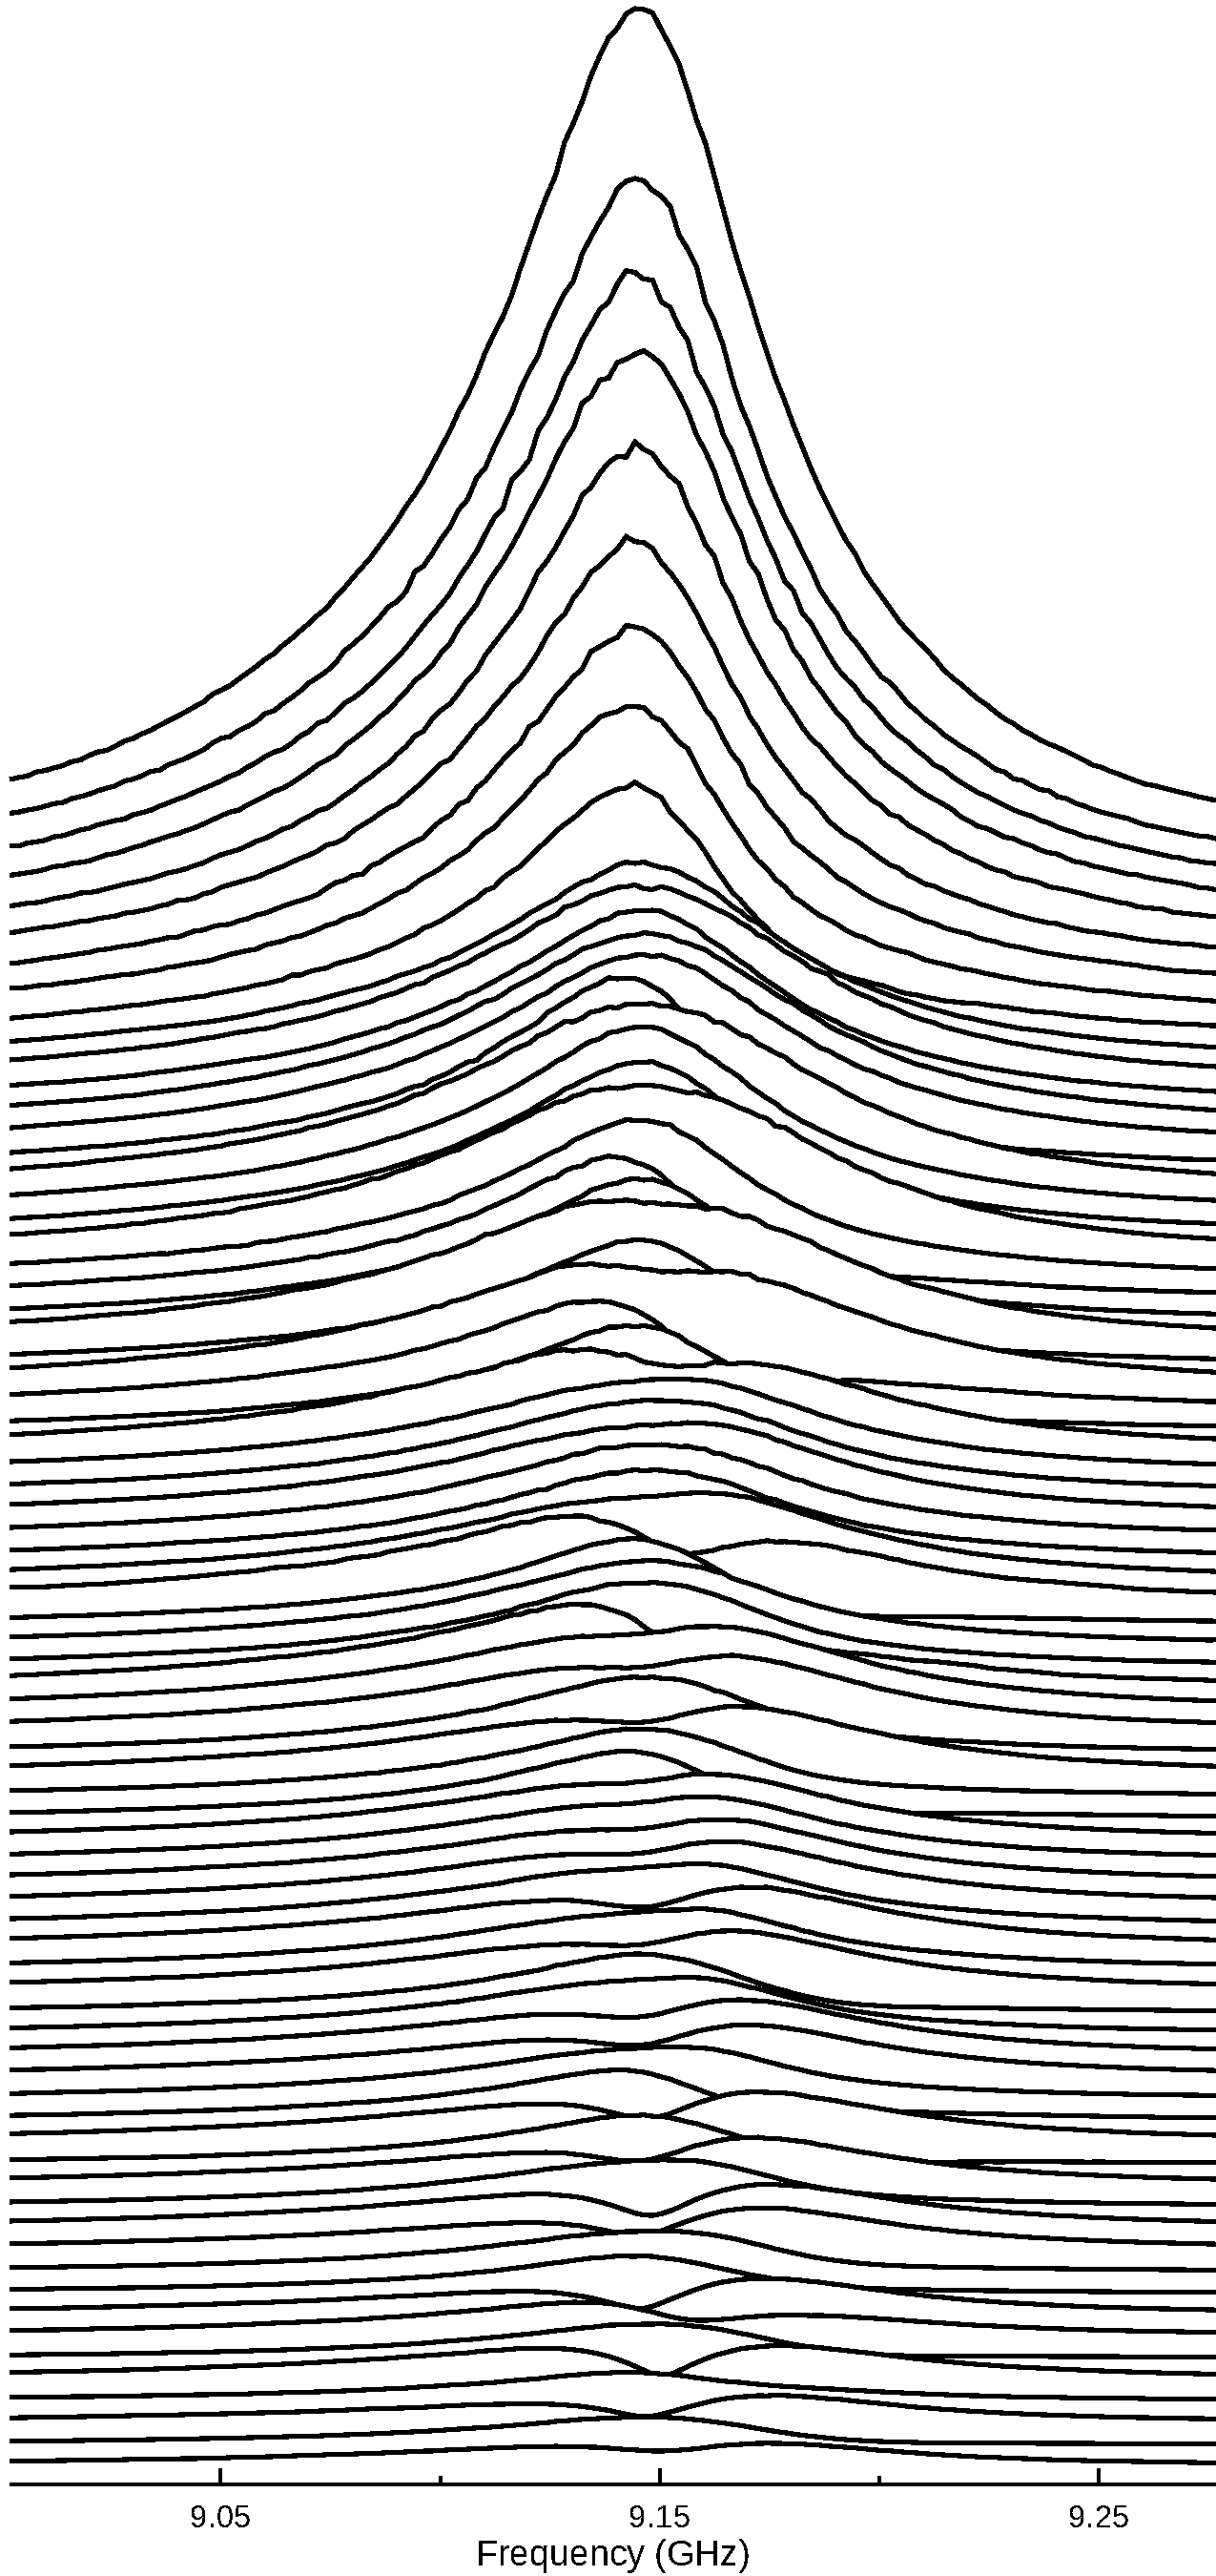
\includegraphics[height=0.90\textheight]{figs/3-CoBS/JoyDivisionCoBSUHNA3.pdf}
\caption[All measured Brillouin spectra for \SI{1}{\centi\meter}~\ac{UHNA3} at pump-probe detuning steps of \SI{0.5}{\giga\hertz} from \SI{5}{\giga\hertz} to \SI{42}{\giga\hertz}.]{All measured Brillouin spectra for \SI{1}{\centi\meter}~\ac{UHNA3} at pump-probe detuning steps of \SI{0.5}{\giga\hertz} from \SI{5}{\giga\hertz} (top spectrum) to \SI{42}{\giga\hertz} (bottom spectrum). Each trace is offset for clarity. The resulting asymmetries highlight the characteristic Fano-resonant behavior under low signal conditions.}
\label{fig:Joy Division UHNA3}
\end{figure}

\FloatBarrier

\subsection{Fano Experiment~B: \SI{1}{\milli\meter} \texorpdfstring{\ce{CS2}}{CS2} Spectra and Fano Distortions}
\label{Appendix:Fano:Experiment B}

We now turn to measurements on a \SI{1}{\milli\meter}-thick cell of \ce{CS2} in a free-space geometry, complementing the \SI{1}{\centi\meter} \ac{UHNA3} fiber results (Experiment~A). Both experiments used comparable sub-Watt optical powers (on the order of \(\sim\)60–\SI{70}{\milli\watt} pump, \(\sim\)25–\SI{30}{\milli\watt} Stokes, and \(\sim\)40–\SI{50}{\milli\watt} probe). However, unlike Experiment~A, which probed a \SI{1}{\centi\meter} fiber with \SI{0.5}{\giga\hertz} detuning increments from \SI{5}{\giga\hertz} to \SI{42}{\giga\hertz}, here the detuning is stepped in \SI{0.25}{\giga\hertz} increments between \SI{10}{\giga\hertz} and \SI{14}{\giga\hertz}. Because the \ce{CS2} sample is an order of magnitude shorter (\SI{1}{\milli\meter} vs.\ \SI{1}{\centi\meter}), its phase-matching bandwidth (\(\mathrm{sinc}^{2}\) profile) is roughly ten times wider, making these \SI{0.25}{\giga\hertz} steps effectively twenty times finer than the \SI{0.5}{\giga\hertz} steps used in the fiber experiment. This reduced range of detunings within a broader \(\mathrm{sinc^2}\) profile produce measured peaks all of similar amplitude to one another, as opposed to the dynamic evolution of peaks in the \SI{1}{\centi\meter} \ac{UHNA3} fiber data.

Figure~\ref{fig:Joy Division CS2} shows all 17 spectra obtained at detuning increments of \SI{0.25}{\giga\hertz}, presented in order of increasing detuning from top spectrum to bottom spectrum. Each trace is offset vertically for clarity, with the topmost spectrum corresponding to \SI{10}{\giga\hertz} and the bottom spectrum corresponding to \SI{14}{\giga\hertz} detuning of the pump and the probe. A change in the detuning of the pump and probe via adjustment of the probe laser wavelength produces a change in phase of the resonant Brillouin signal. This changing resonant Brillouin phase relative to the background continuum produces spectra with different Fano-resonant distortions corresponding to specific values of the Fano parameter, \(q\), as discussed in \textit{Fano-Resonant Asymmetries at Small Signals} in the main text (Section~\ref{Results:Fano-Resonant Asymmetries at Small Signals}). Fano-resonant asymmetries are seen in nearly every spectrum of this liquid experiment, indicating that the background continuum is competing strongly with the Brillouin amplitude in all measurements.

The Brillouin amplitudes featured in this experiment are an order of magnitude lower compared to the highest amplitudes seen in Experiment~A. This is caused by the order of magnitude shorter sample length of \ce{CS2} (\SI{1}{\milli\meter}) as compared to the \SI{1}{\centi\meter} length of \ac{UHNA3} fiber used in Experiment~A. The \(\sim\)1000 times higher Brillouin gain offered by the \ce{CS2} (\SI{1.5}{\meter\per\giga\watt}) is discounted significantly by the \(\sim\)350 times larger effective area offered by the beam waist in the free-space optical setup compared to the core of \ac{UHNA3} fiber used in Experiment~A (\(\sim\)\SI{17}{\micro\meter} radius beam waist vs. \(\sim\)\SI{0.9}{\micro\meter} radius core of UHNA3). The effective Brillouin gain of the \ce{CS2} used in Experiment~B is thus a net \(\sim\)3 times greater than that of the \ac{UHNA3} fiber. From Equations~\ref{Eq:Theoretical Framework:Scattered Power} and \ref{Eq:Effective Brillouin Gain} in the main text, scattered power scales with the square of both the length and the effective Brillouin gain of the sample (\(P_{\rm Sig} \propto L^{2}G_{\rm B}^{2}\)). Cumulatively, this makes for an approximate order-of-magnitude signal reduction for similar optical powers and pump-probe detuning.

However, both experiments (A and B) feature a sweep through a range of pump-probe detunings, with Experiment~B featuring a step size effectively 25 times finer than that of Experiment~A. This further corroborates these two data sets, as the signal reduction from near-center peak to a side trough of the \(\mathrm{sinc^{2}}\) profile is also on the order of a 10 times reduction (Figure~\ref{fig:Phase-Match}). This places the signal amplitudes of the \ce{CS2} spectra from Experiment~B (all near \textit{peak-center} of its \(\mathrm{sinc^{2}}\) profile) on the same order as the signal amplitudes near the \textit{troughs} of the UHNA3 fiber spectra from Experiment~A. These spectra all share strong Fano asymmetries, indicating as they should that they all sit in a similar signal amplitude range: small enough that the background continuum competes but does not dominate over the signal.

\begin{figure}[ht]
  \centering
  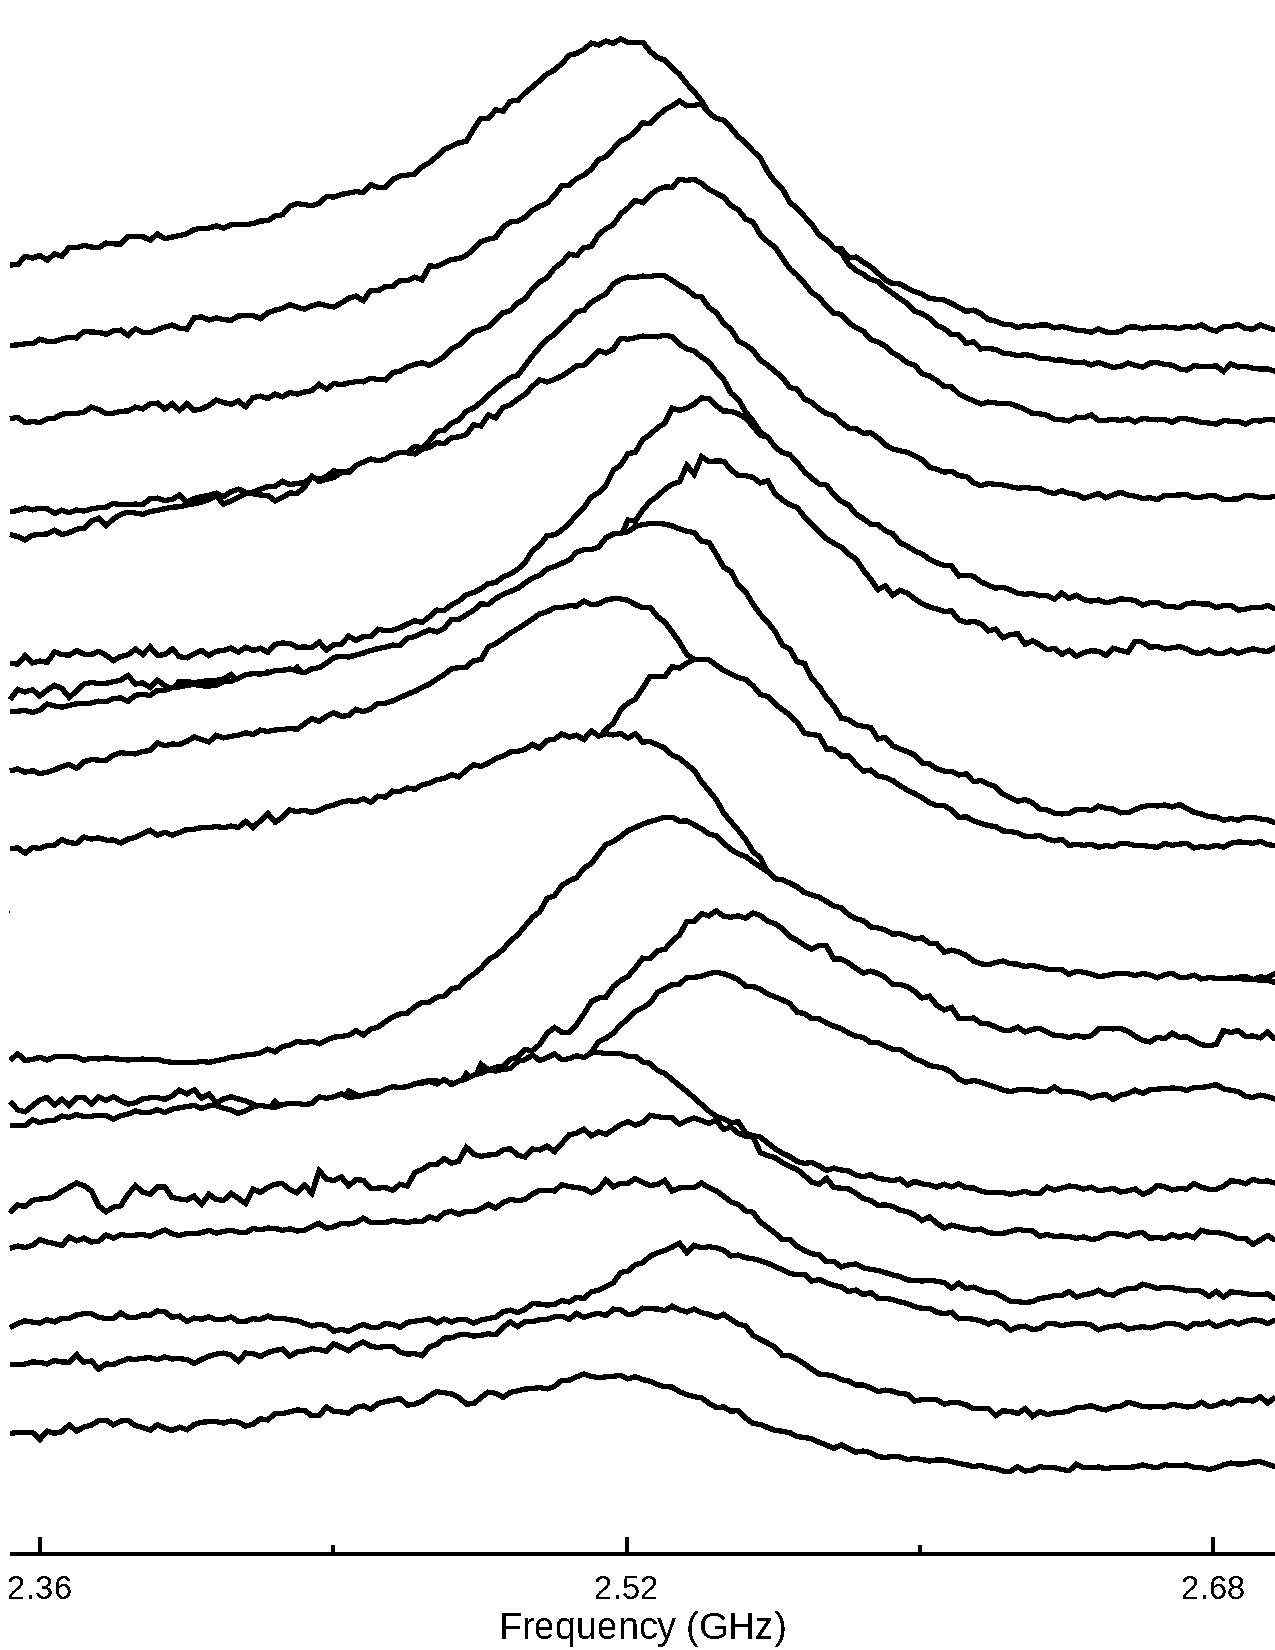
\includegraphics[width=0.7\textwidth]{figs/3-CoBS/JoyDivisionCoBSCS2.pdf}
  \caption[All measured Brillouin spectra for \SI{1}{\milli\meter}~\ce{CS2} at pump-probe detuning steps of \SI{0.25}{\giga\hertz} from \SI{10}{\giga\hertz} to \SI{14}{\giga\hertz}.]{All measured Brillouin spectra for \SI{1}{\milli\meter}~\ce{CS2} at pump-probe detuning steps of \SI{0.25}{\giga\hertz} from \SI{10}{\giga\hertz} (top spectrum) to \SI{14}{\giga\hertz} (bottom spectrum). Each trace is offset for clarity.}
  \label{fig:Joy Division CS2}
\end{figure}

\FloatBarrier

To illustrate the strong distinction in line-shape of a spectra resulting from a positive vs. negative \(q\) value, we focus on two particular detunings that yielded notably skewed line shapes: \SI{11}{\giga\hertz} and \SI{13}{\giga\hertz}. Figures~\ref{fig:CS2FanoCompare} and \ref{fig:CS2LorentzCompare} compare the spectra for these two detunings normalized relative to the slightly larger peak amplitude of the \SI{11}{\giga\hertz} spectra. The line-shape of the \SI{11}{\giga\hertz} spectrum exhibits a sharper rise on the higher-frequency side and a gentler roll-off on the lower-frequency side, indicative of \(q<0\), whereas that of the \SI{13}{\giga\hertz} spectrum is skewed oppositely, featuring a sharper low-frequency side and a softer high-frequency roll-off, suggesting \(q>0\). Figure~\ref{fig:CS2FanoCompare} shows these two spectra with uncertainty-weighted Fano function fits applied, with the corresponding reduced \(\chi^{2}\) values reported in the legend. The Fano fits yield reduced \(\chi^{2}\) values of 2.45 and 8.41 for the \SI{11}{\giga\hertz} and \SI{13}{\giga\hertz} spectra, respectively (reduced \(\chi^{2}\) values near unity indicate a good fit to the data). Figure~\ref{fig:CS2LorentzCompare} shows these same spectra with naïve Lorentz function fits applied and their corresponding reduced \(\chi^{2}\) evaluations of goodness-of-fit. These Lorentzian fits yield reduced \(\chi^{2}\) values of 39.45 and 146.5 for the \SI{11}{\giga\hertz} and \SI{13}{\giga\hertz} spectra, respectively, indicating that the Lorentzian function is a very poor fit to the data.. The poor fit of the Lorentzian function is due to its inherent symmetry, whereas the underlying data exhibit strongly asymmetric lineshapes. These results clearly demonstrate the superiority of the Fano model in capturing the asymmetry of small signals produced by the instrument due to Fano interference with the background continuum. This, in turn, emphasizes the importance of applying a Fano fit function when asymmetries arise to accurately extract valuable spectra parameters such as peak amplitude, center frequency, and linewidth from the data.

Notably, in the \(\SI{11}{\giga\hertz}\) case, our Fano fit reveals a local amplitude slightly higher than what the Lorentzian fit suggests, sometimes referred to as a “peak boost.” In essence, partial \emph{constructive} interference between the discrete Brillouin response and the broad continuum locally raises the amplitude, although it does not imply any net energy gain. As mentioned in \textit{Fano-Resonant Asymmetries at Small Signals} (Section~\ref{Results}), this effect can aid in detecting weak resonances if the background is not too noisy. One could, in principle, tune the phase relationship to maximize this interference near the resonance, possibly producing a sharper or taller peak for certain values of \(q\) than would be achieved without interference with the background. This Fano interference-tuning of the discrete mode relative to the background can be done dynamically via adjustment of the probe laser wavelength and, critically, can be adjusted independently from the phase-matching bandwidth tuning (pump-probe detuning). This is ability to dynamically adjust the discrete-continuum interference is an elegant and notable feature, as in typical systems this is adjusted via changes in physical geometry or material doping of the sample.\cite{ko2023full, gu2020fano, rieger2023fano}

\begin{figure}[ht]
  \centering
  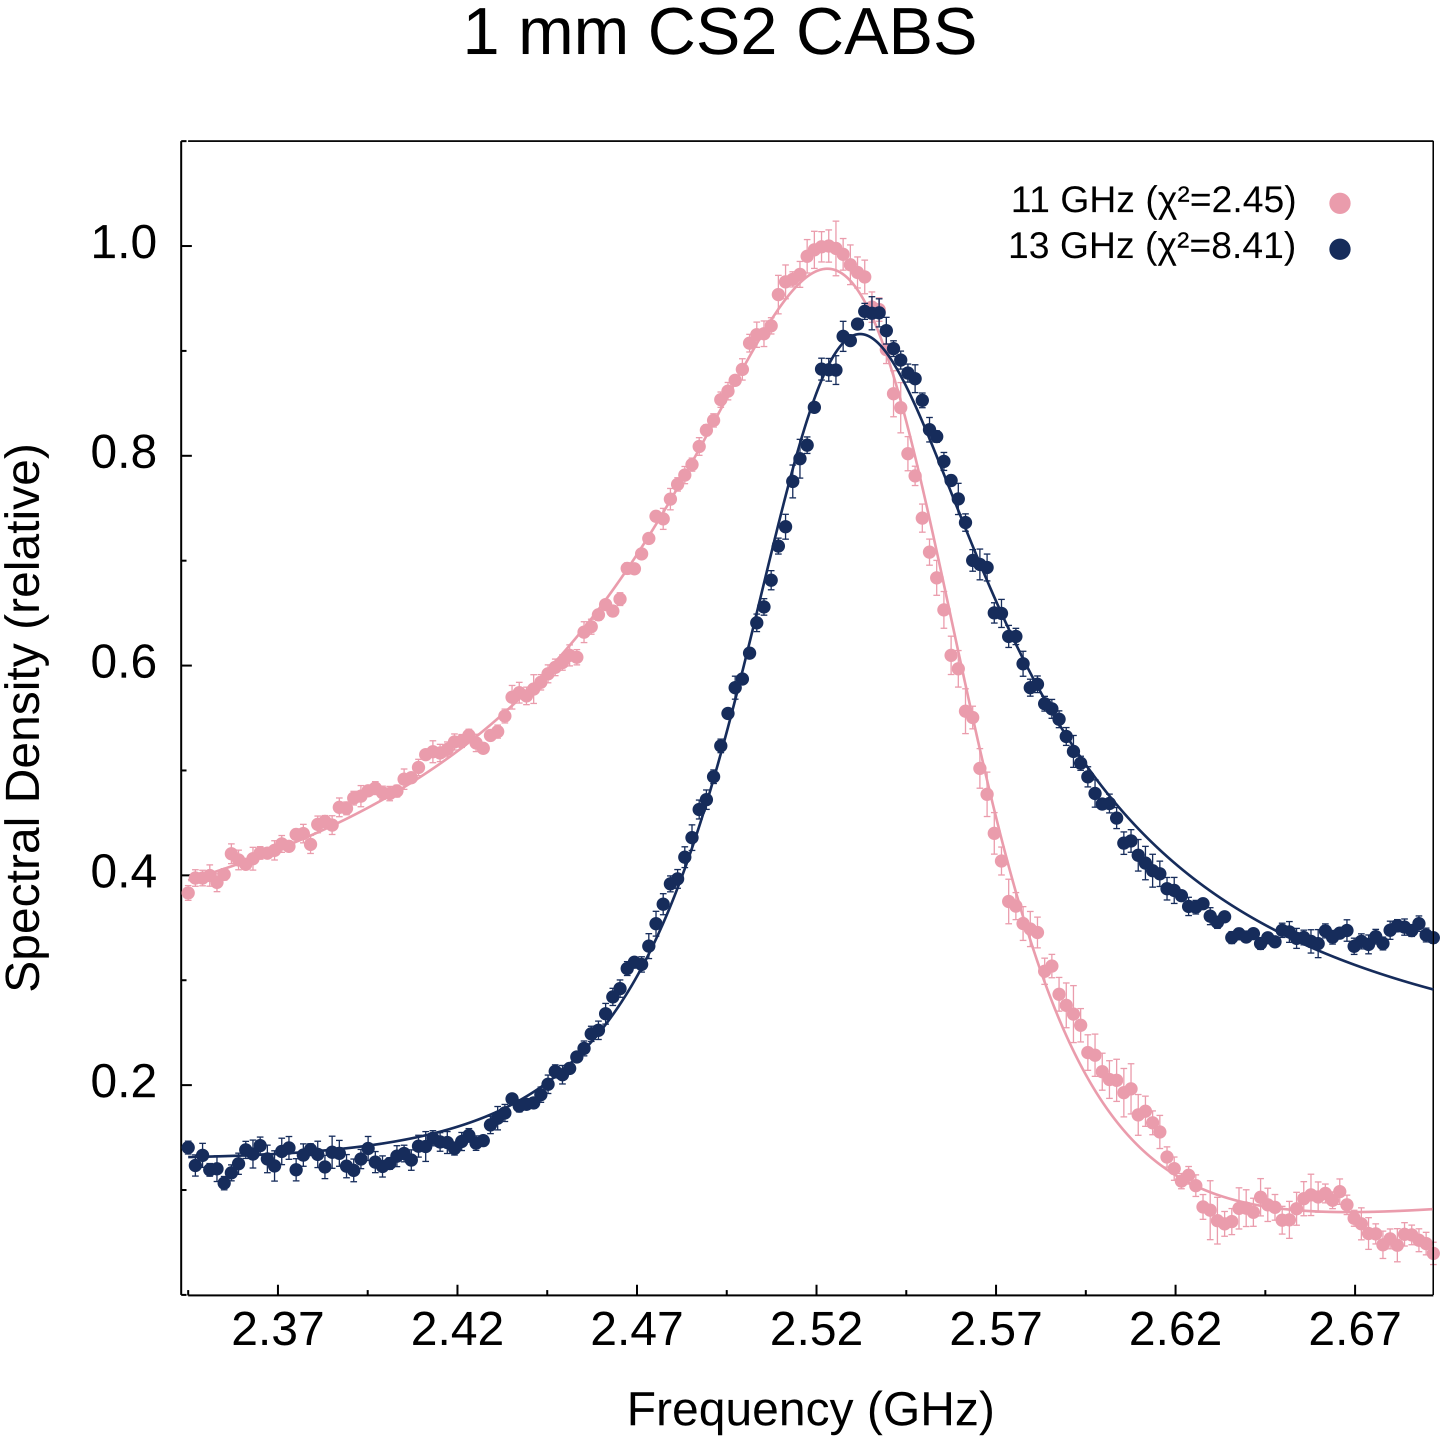
\includegraphics[width=\textwidth]{figs/3-CoBS/CS2FanoCompare.png}
  \caption[Comparison of representative spectra at \SI{11}{\giga\hertz} and \SI{13}{\giga\hertz}, showing the positive vs. negative \(q\) asymmetry in \SI{1}{\milli\meter} \ce{CS2}, with a Fano fit applied.]{Comparison of representative spectra at \SI{11}{\giga\hertz} and \SI{13}{\giga\hertz}, showing the positive vs. negative \(q\) asymmetry in \SI{1}{\milli\meter} \ce{CS2}. A Fano function fit has been applied to each spectra, with \(\chi^{2}\) value for each fit listed in the plot legend.}
  \label{fig:CS2FanoCompare}
\end{figure}

\begin{figure}[ht]
  \centering
  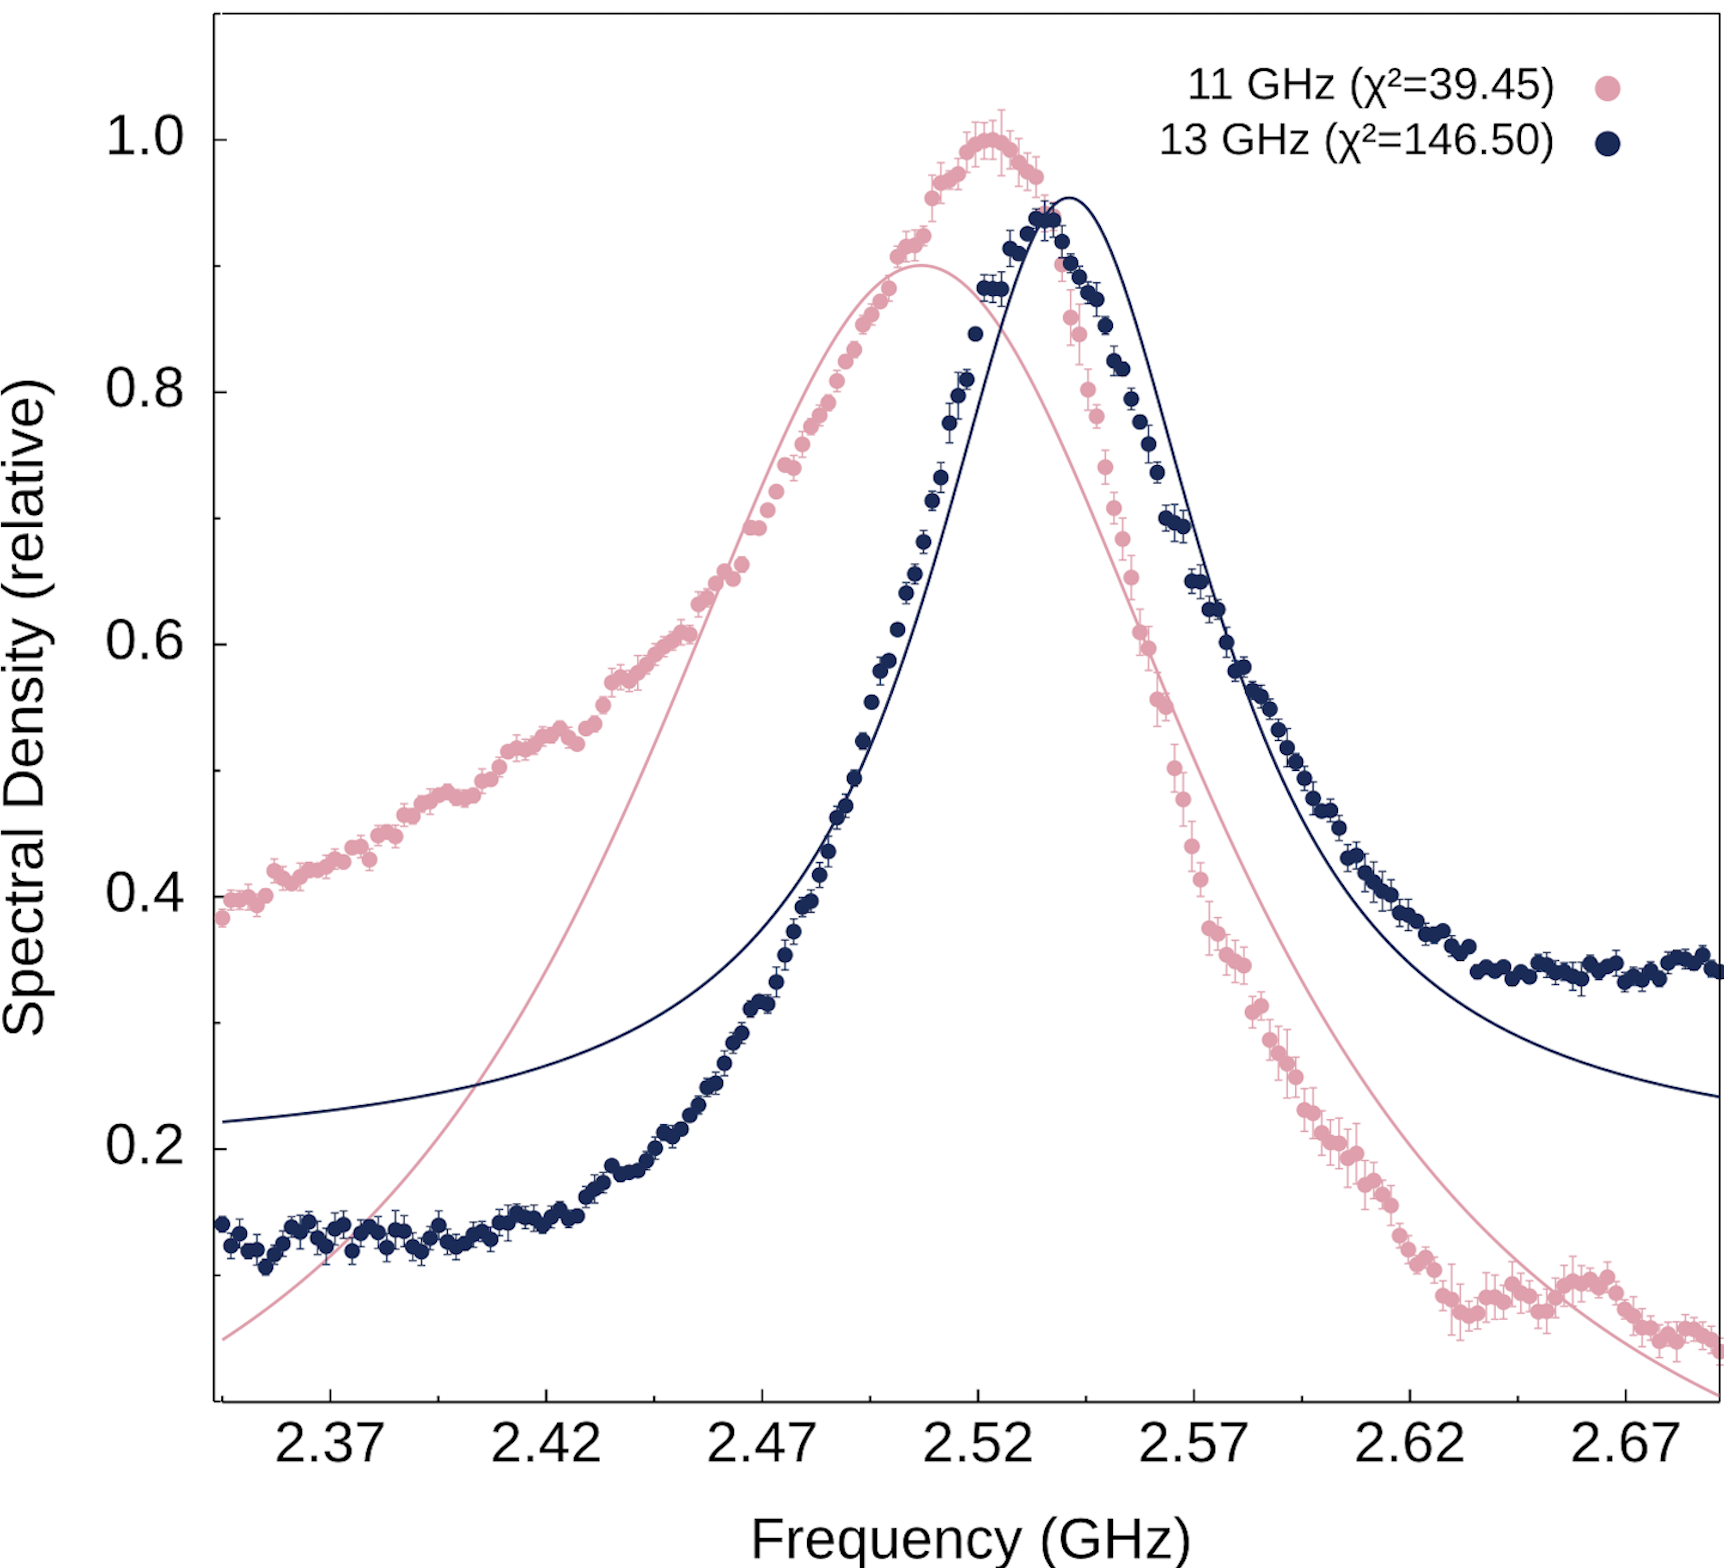
\includegraphics[width=\textwidth]{figs/3-CoBS/CS2LorentzCompare.png}
  \caption[Comparison of representative spectra at \SI{11}{\giga\hertz} and \SI{13}{\giga\hertz}, showing the positive vs.\ negative \(q\) asymmetry in \SI{1}{\milli\meter} \ce{CS2}, with a naïve Lorentz fit applied.]{Comparison of representative spectra at \SI{11}{\giga\hertz} and \SI{13}{\giga\hertz}, showing the positive vs.\ negative \(q\) asymmetry in \SI{1}{\milli\meter} \ce{CS2}. Here, a naïve Lorentz function fit has been applied to each spectra, with \(\chi^{2}\) value for each fit listed in the plot legend. These spectra show strong Fano-resonant asymmetry and thus the standard Lorentz function offers a poor fit for these spectra, quantified by the \(\chi^{2}\) evaluation metric for goodness of fit as compared to the same evaluation of the Fano function fit.}
  \label{fig:CS2LorentzCompare}
\end{figure}

\FloatBarrier

To better convey the cyclical evolution of the 75 measured UHNA3 spectra from Experiment~A, several animated GIFs have been generated. The following is a link to the GitHub repository which hosts these files, along with all raw data, measurement logs, and plots generated in support of this work (see See Appendix~\ref{appendix:CodeandDataAvailability}):

\hfill

\begin{center}
  \url{https://github.com/HamletTheHamster/Plotting-Data-in-Go}
\end{center}

\hfill

The reader will find several GIFs which step through each spectrum in ascending pump--probe detuning at various frame rates. Readers are encouraged to view them for an animated perspective on how the spectra evolve with increasing pump--probe detuning, with special attention to transitions between Lorentzian and Fano-distorted line shapes.

\newpage

%------------------------------------------------------------------------------%

\section{CoBS Mini Experiment: Equal Contribution of Pump, Stokes, and Probe}

Equation~\ref{Eq:Theoretical Framework:Scattered Power} gives the somewhat unintuitive result that the powers of the Pump, Stokes, and Probe waves contribute equally to the resulting scattered power of the Signal and invites verification with a miniexperiment. Initially, this experiment was motivated by a practical consideration: determination of whether the placement of a high power amplifier on any specific line of the setup (Pump, Stokes, or Probe) would offer any advantage over another.

To test this, we conducted a controlled experiment with a \SI{1}{\milli\meter} \ce{CS2} sample. For each measurement, one of the three source powers (Pump, Stokes, or Probe) was systematically reduced by 75\% while holding the others constant and ensuring consistent experimental conditions across trials. Table~\ref{tab:PSPr-Contribute-Equally} shows the respective powers for each source during the three measurements, along with the multiplicative total contribution of the three powers for each measurement towards the generation of scattered power of the Signal.

\begin{table}[ht]
  \centering
  \renewcommand{\arraystretch}{1.2}
  \begin{tabular}{>{\centering\arraybackslash}m{2.5cm}>{\centering\arraybackslash}m{2.5cm}>{\centering\arraybackslash}m{2.5cm}>{\centering\arraybackslash}m{2.5cm}>{\centering\arraybackslash}m{2.5cm}}
    \toprule
    \shortstack{\rule{0pt}{2.5mm} \\ \textbf{Measurement} \\ \rule{0pt}{2.5mm}} &
    \shortstack{\textbf{Pump Power} \\ (\si{\milli\watt})} &
    \shortstack{\textbf{Stokes Power} \\ (\si{\milli\watt})} &
    \shortstack{\textbf{Probe Power} \\ (\si{\milli\watt})} &
    \shortstack{\textbf{Total} \\ (\si{\milli\watt\cubed})} \\
    \midrule
    Pump Lower & 19.190 & 32.210 & 54.560 & 3.372 \(\times 10^{4}\) \\
    Stokes Lower & 76.600 & 8.020 & 54.650 & 3.359 \(\times 10^{4}\) \\
    Probe Lower & 76.600 & 32.530 & 13.480 & 3.359 \(\times 10^{4}\) \\
    \bottomrule
  \end{tabular}
    \caption{Power values for each source (Pump, Stokes, Probe) across the three measurements, with the multiplicative total power for each setup.}
    \label{tab:PSPr-Contribute-Equally}
\end{table}

Figure~\ref{fig:PSPr-Contribute-Equally} displays the average results from these three measurements, plotted with error bars representing one standard deviation of the mean. For increased certainty, Figure~\ref{fig:PSPr-Contribute-Equally-2sigma} presents the same data with error bars extended to two standard deviations, providing additional confidence in the reproducibility of the results. This experiment confirms that the scattered Signal power indeed depends equally on each of the three contributing wave powers, as expected from the theoretical framework. Consequently, boosting the power of any of the three sources affects the Signal power equally, allowing flexibility in pragmatic design across any of the three lines. Ultimately, this result reinforces the reliability of Equation~\ref{Eq:Theoretical Framework:Scattered Power} for predicting Signal power across a range of power distributions within practical settings.

\begin{figure}[ht]
  \centering
  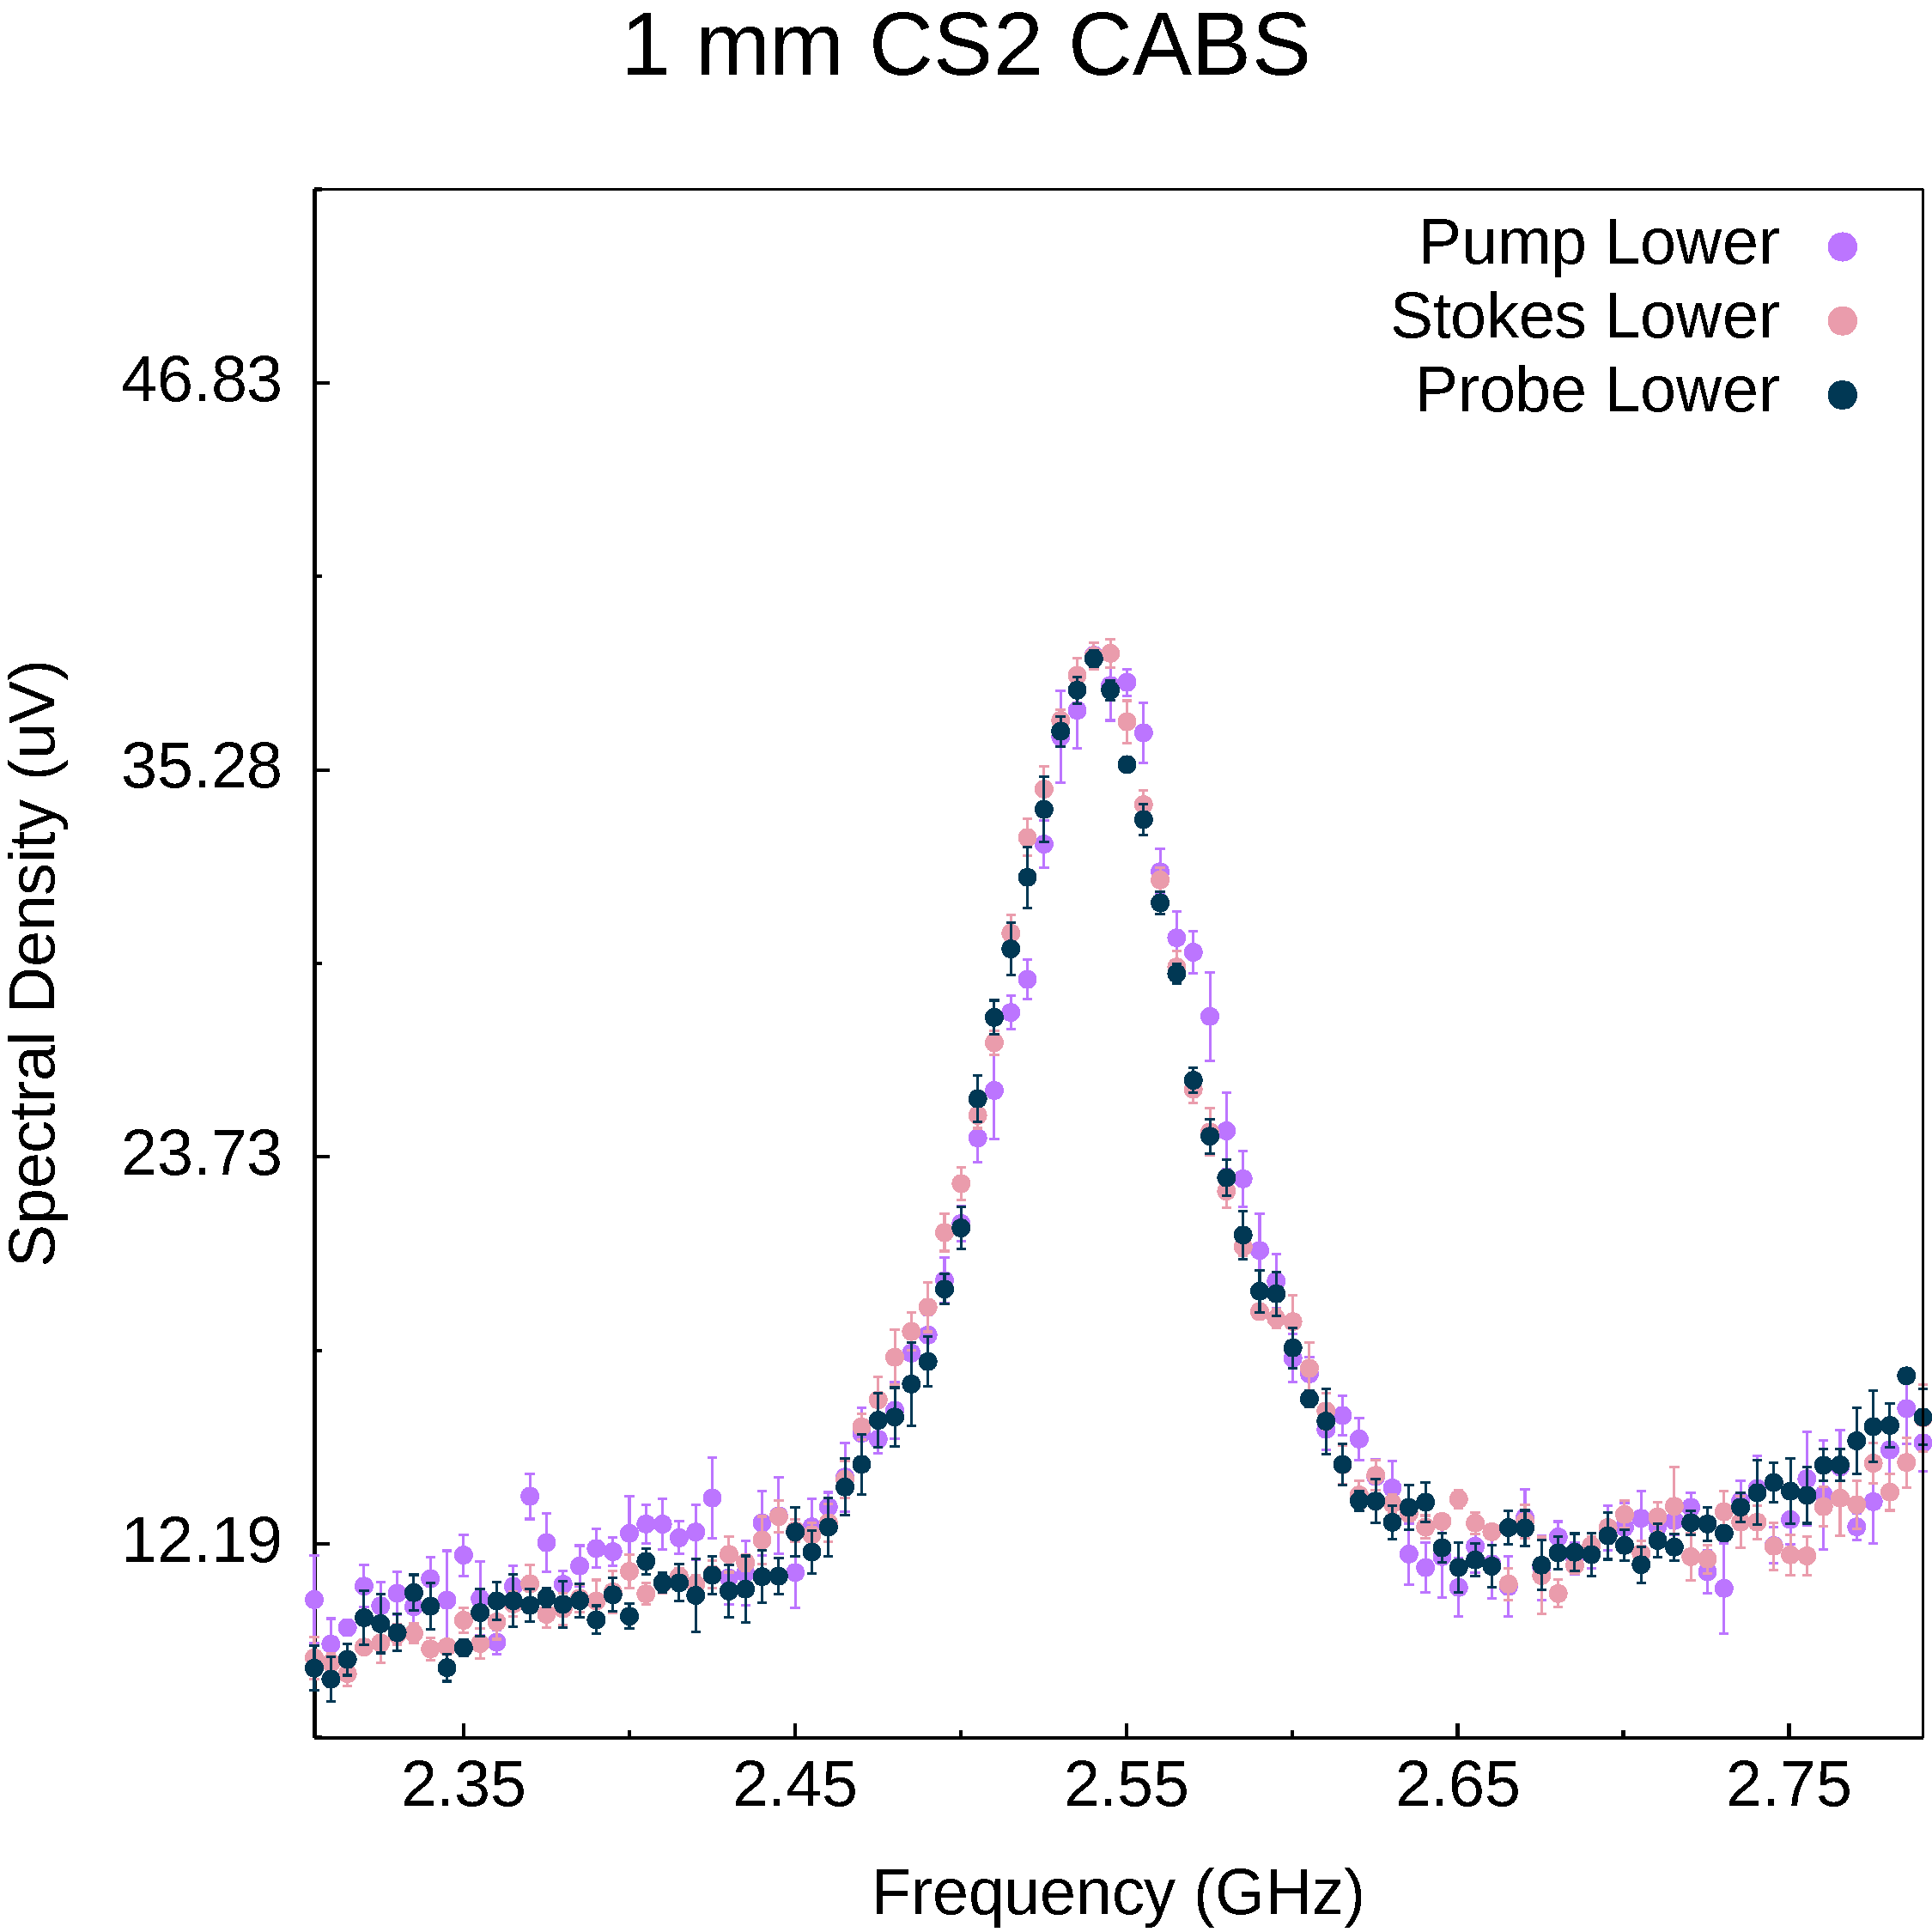
\includegraphics[width=\textwidth]{figs/3-CoBS/PSPr-Contribute-Equally.pdf}
  \caption{Scattered power spectra with varying proportions of pump, Stokes, and probe power and error bars representing one standard deviation of the mean for each measurement.}
  \label{fig:PSPr-Contribute-Equally}
\end{figure}

\begin{figure}[ht]
  \centering
  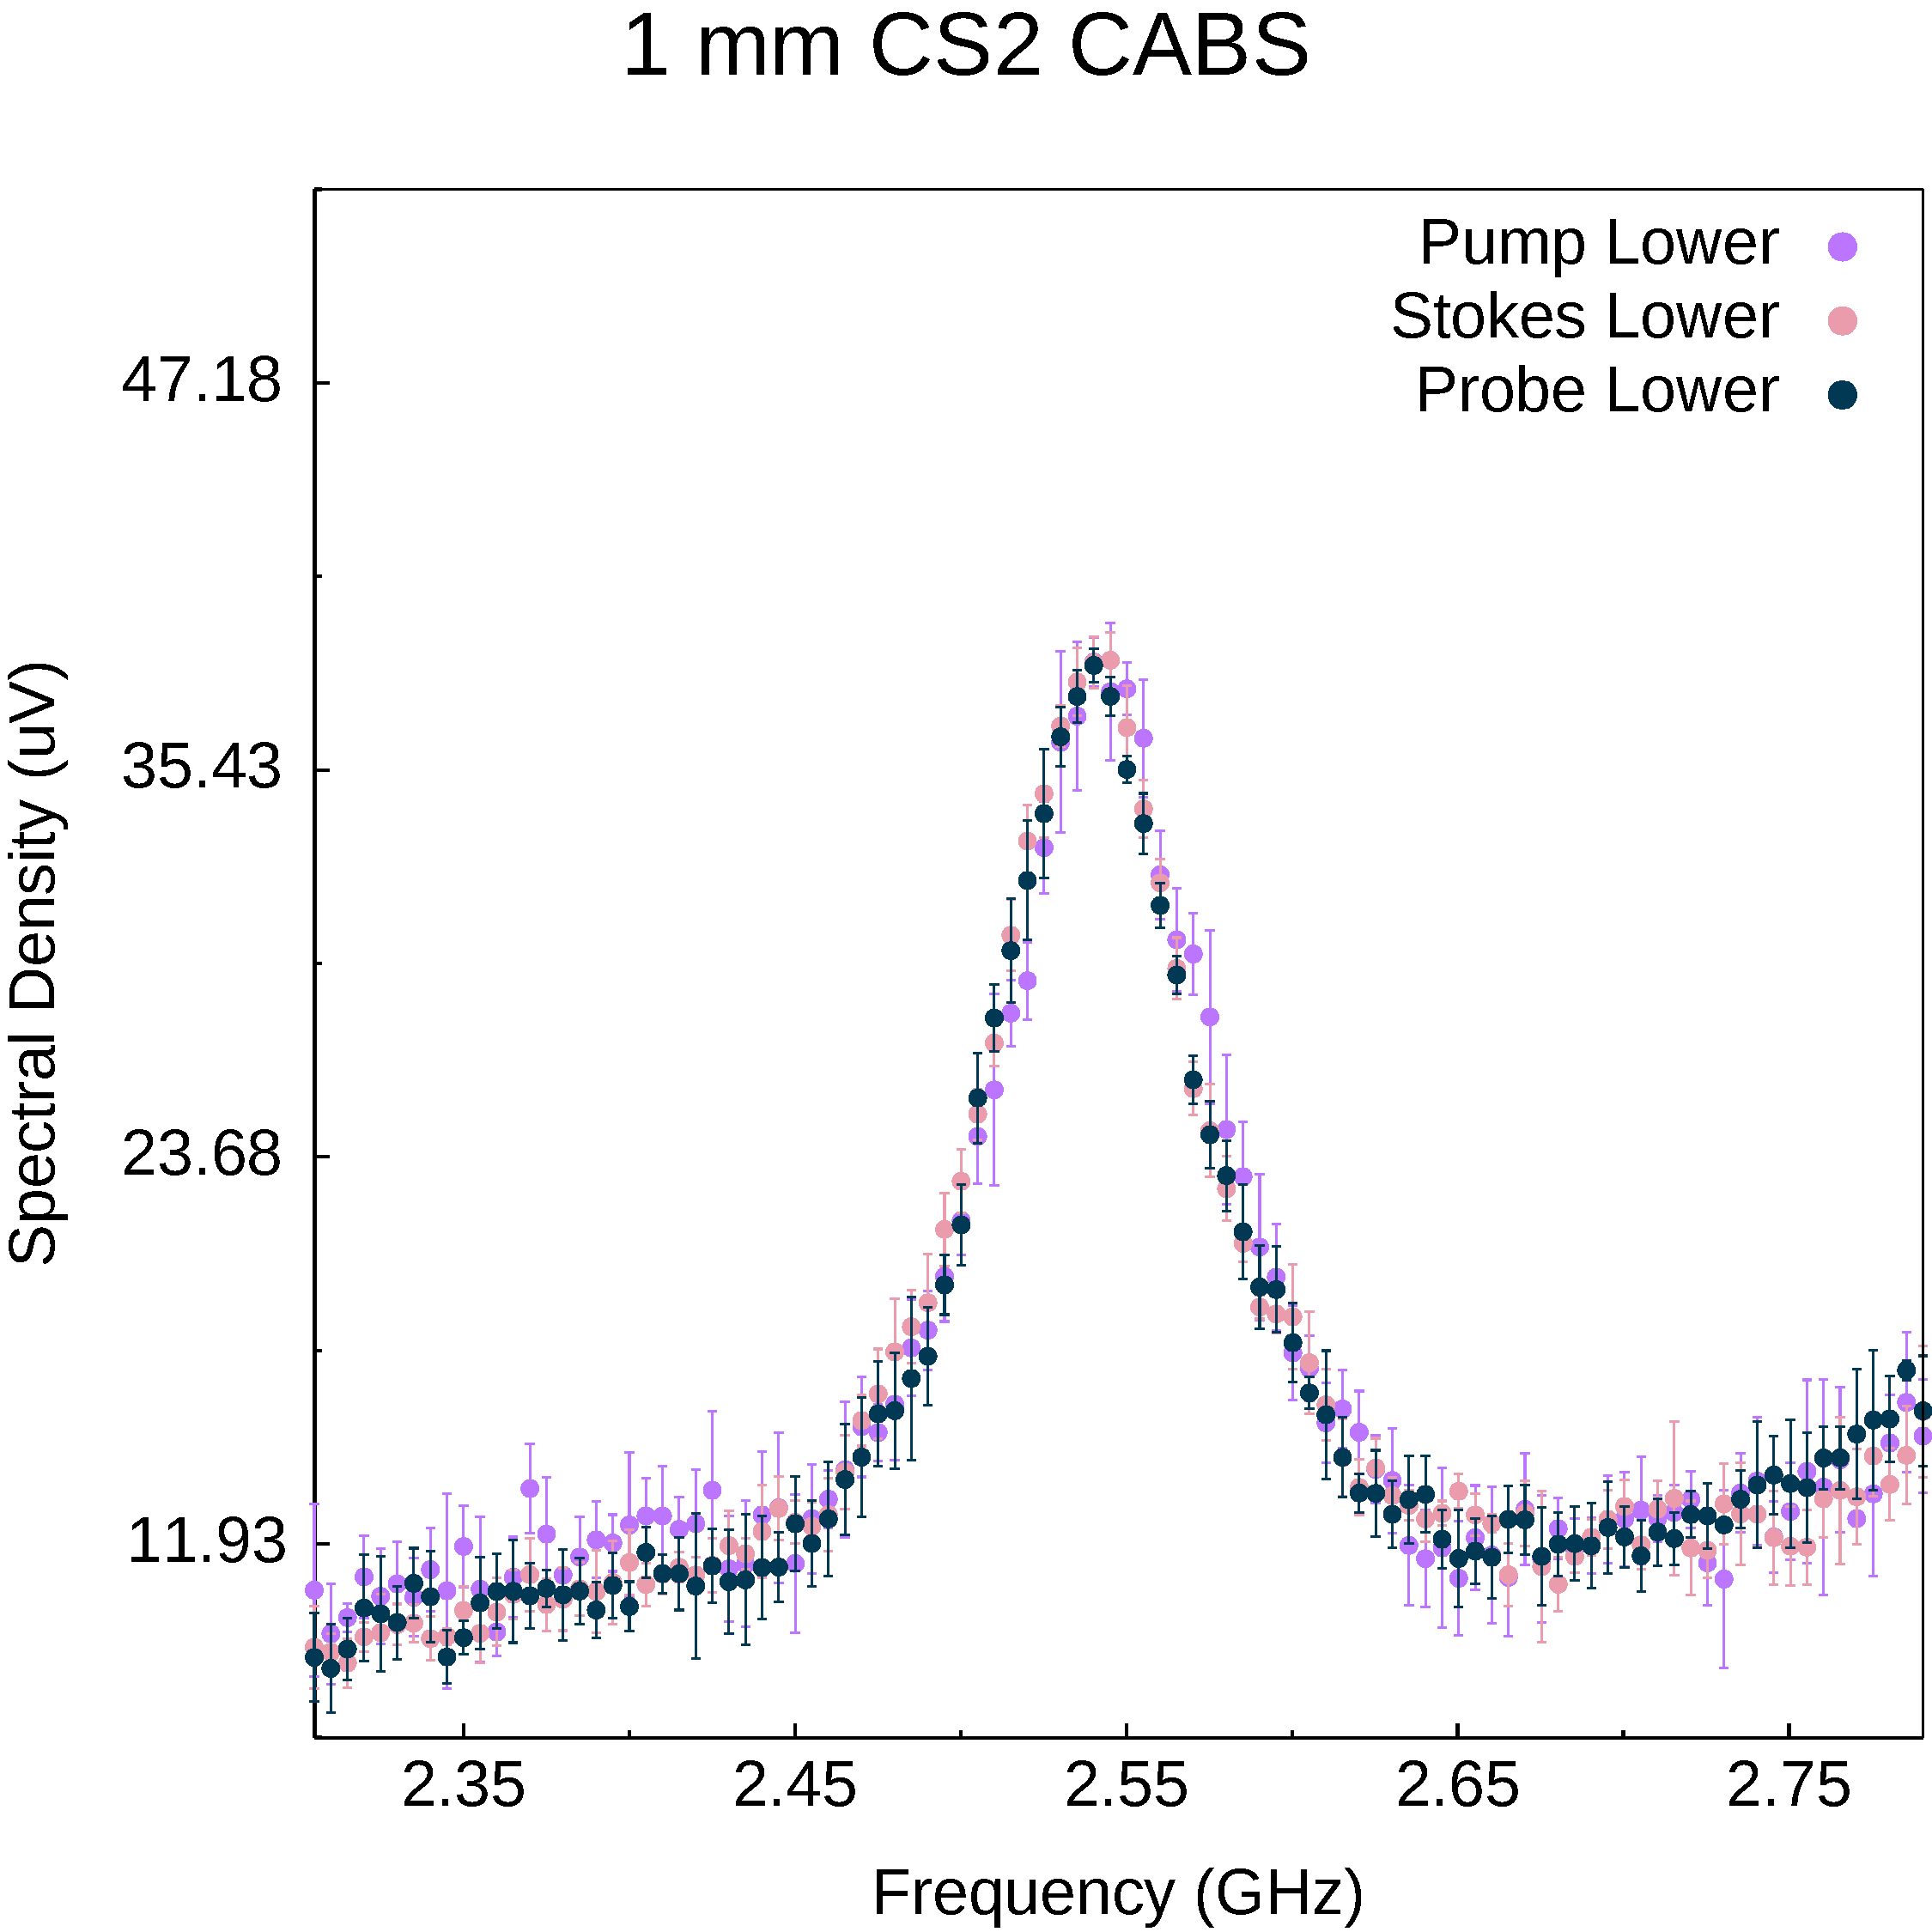
\includegraphics[width=\textwidth]{figs/3-CoBS/PSPr-Contribute-Equally-2sigma.pdf}
  \caption{Scattered power spectra with varying proportions of pump, Stokes, and probe power and error bars extended to two standard deviations of the mean for each measurement.}
  \label{fig:PSPr-Contribute-Equally-2sigma}
\end{figure}

\FloatBarrier

\newpage

% \section{Measurement Protocol}
% \label{CoBS:Appendix:sec:MeasurementProtocol}
